% Created by tikzDevice version 0.12 on 2019-05-09 12:17:50
% !TEX encoding = UTF-8 Unicode
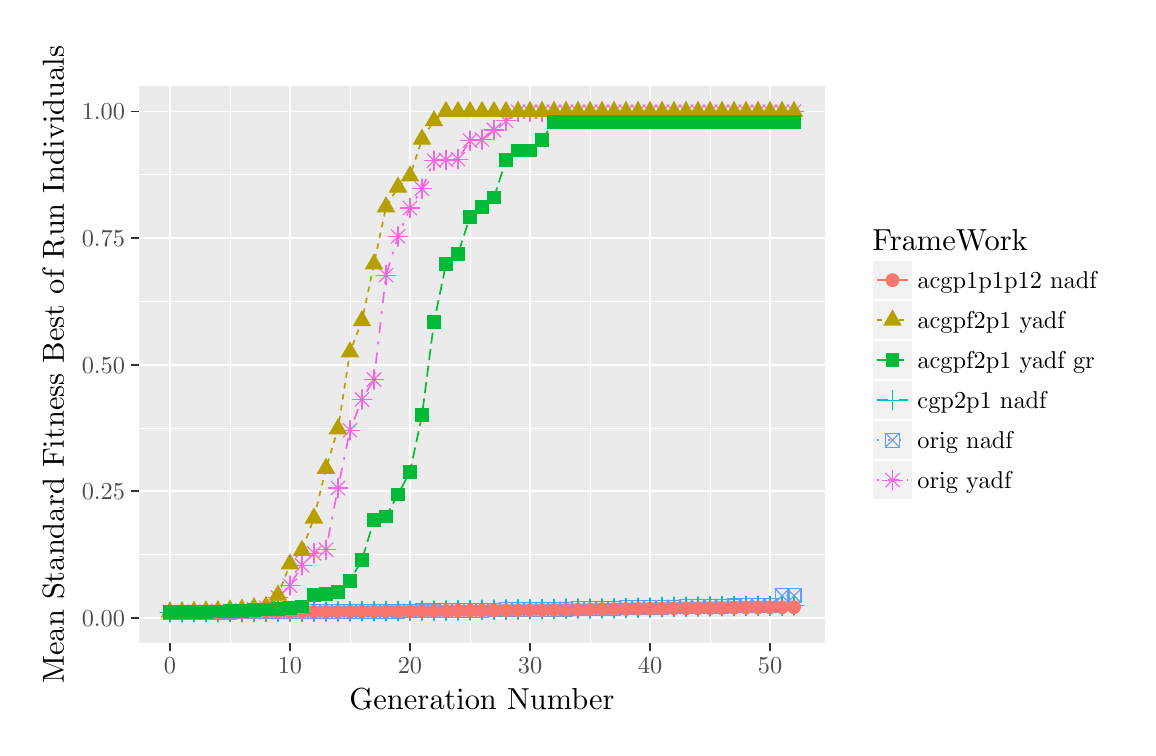
\begin{tikzpicture}[x=1pt,y=1pt]
\definecolor{fillColor}{RGB}{255,255,255}
\path[use as bounding box,fill=fillColor,fill opacity=0.00] (0,0) rectangle (397.48,252.94);
\begin{scope}
\path[clip] (  0.00,  0.00) rectangle (397.48,252.94);
\definecolor{drawColor}{RGB}{255,255,255}
\definecolor{fillColor}{RGB}{255,255,255}

\path[draw=drawColor,line width= 0.6pt,line join=round,line cap=round,fill=fillColor] (  0.00,  0.00) rectangle (397.48,252.95);
\end{scope}
\begin{scope}
\path[clip] ( 40.14, 30.56) rectangle (288.20,231.75);
\definecolor{fillColor}{gray}{0.92}

\path[fill=fillColor] ( 40.14, 30.56) rectangle (288.20,231.75);
\definecolor{drawColor}{RGB}{255,255,255}

\path[draw=drawColor,line width= 0.3pt,line join=round] ( 40.14, 62.57) --
	(288.20, 62.57);

\path[draw=drawColor,line width= 0.3pt,line join=round] ( 40.14,108.29) --
	(288.20,108.29);

\path[draw=drawColor,line width= 0.3pt,line join=round] ( 40.14,154.02) --
	(288.20,154.02);

\path[draw=drawColor,line width= 0.3pt,line join=round] ( 40.14,199.75) --
	(288.20,199.75);

\path[draw=drawColor,line width= 0.3pt,line join=round] ( 73.10, 30.56) --
	( 73.10,231.75);

\path[draw=drawColor,line width= 0.3pt,line join=round] (116.47, 30.56) --
	(116.47,231.75);

\path[draw=drawColor,line width= 0.3pt,line join=round] (159.83, 30.56) --
	(159.83,231.75);

\path[draw=drawColor,line width= 0.3pt,line join=round] (203.20, 30.56) --
	(203.20,231.75);

\path[draw=drawColor,line width= 0.3pt,line join=round] (246.57, 30.56) --
	(246.57,231.75);

\path[draw=drawColor,line width= 0.6pt,line join=round] ( 40.14, 39.70) --
	(288.20, 39.70);

\path[draw=drawColor,line width= 0.6pt,line join=round] ( 40.14, 85.43) --
	(288.20, 85.43);

\path[draw=drawColor,line width= 0.6pt,line join=round] ( 40.14,131.16) --
	(288.20,131.16);

\path[draw=drawColor,line width= 0.6pt,line join=round] ( 40.14,176.88) --
	(288.20,176.88);

\path[draw=drawColor,line width= 0.6pt,line join=round] ( 40.14,222.61) --
	(288.20,222.61);

\path[draw=drawColor,line width= 0.6pt,line join=round] ( 51.41, 30.56) --
	( 51.41,231.75);

\path[draw=drawColor,line width= 0.6pt,line join=round] ( 94.78, 30.56) --
	( 94.78,231.75);

\path[draw=drawColor,line width= 0.6pt,line join=round] (138.15, 30.56) --
	(138.15,231.75);

\path[draw=drawColor,line width= 0.6pt,line join=round] (181.52, 30.56) --
	(181.52,231.75);

\path[draw=drawColor,line width= 0.6pt,line join=round] (224.88, 30.56) --
	(224.88,231.75);

\path[draw=drawColor,line width= 0.6pt,line join=round] (268.25, 30.56) --
	(268.25,231.75);
\definecolor{drawColor}{RGB}{248,118,109}

\path[draw=drawColor,line width= 0.6pt,line join=round] ( 51.41, 41.70) --
	( 55.75, 41.72) --
	( 60.09, 41.73) --
	( 64.42, 41.73) --
	( 68.76, 41.75) --
	( 73.10, 41.75) --
	( 77.43, 41.76) --
	( 81.77, 41.78) --
	( 86.11, 41.79) --
	( 90.44, 41.81) --
	( 94.78, 41.81) --
	( 99.12, 41.82) --
	(103.45, 41.83) --
	(107.79, 41.85) --
	(112.13, 41.86) --
	(116.47, 41.89) --
	(120.80, 41.91) --
	(125.14, 41.93) --
	(129.48, 41.97) --
	(133.81, 41.99) --
	(138.15, 42.01) --
	(142.49, 42.06) --
	(146.82, 42.11) --
	(151.16, 42.18) --
	(155.50, 42.22) --
	(159.83, 42.26) --
	(164.17, 42.29) --
	(168.51, 42.36) --
	(172.84, 42.40) --
	(177.18, 42.44) --
	(181.52, 42.48) --
	(185.85, 42.51) --
	(190.19, 42.56) --
	(194.53, 42.57) --
	(198.86, 42.61) --
	(203.20, 42.70) --
	(207.54, 42.80) --
	(211.87, 42.83) --
	(216.21, 42.86) --
	(220.55, 42.93) --
	(224.88, 42.97) --
	(229.22, 43.03) --
	(233.56, 43.12) --
	(237.89, 43.13) --
	(242.23, 43.15) --
	(246.57, 43.20) --
	(250.90, 43.26) --
	(255.24, 43.35) --
	(259.58, 43.42) --
	(263.91, 43.45) --
	(268.25, 43.48) --
	(272.59, 43.50) --
	(276.92, 43.53);
\definecolor{drawColor}{RGB}{183,159,0}

\path[draw=drawColor,line width= 0.6pt,dash pattern=on 2pt off 2pt ,line join=round] ( 51.41, 41.77) --
	( 55.75, 41.86) --
	( 60.09, 42.03) --
	( 64.42, 42.13) --
	( 68.76, 42.27) --
	( 73.10, 42.50) --
	( 77.43, 42.79) --
	( 81.77, 43.32) --
	( 86.11, 43.78) --
	( 90.44, 47.86) --
	( 94.78, 59.15) --
	( 99.12, 64.00) --
	(103.45, 75.72) --
	(107.79, 93.66) --
	(112.13,107.96) --
	(116.47,135.72) --
	(120.80,146.99) --
	(125.14,167.53) --
	(129.48,188.18) --
	(133.81,195.31) --
	(138.15,199.33) --
	(142.49,212.63) --
	(146.82,219.28) --
	(151.16,222.61) --
	(155.50,222.61) --
	(159.83,222.61) --
	(164.17,222.61) --
	(168.51,222.61) --
	(172.84,222.61) --
	(177.18,222.61) --
	(181.52,222.61) --
	(185.85,222.61) --
	(190.19,222.61) --
	(194.53,222.61) --
	(198.86,222.61) --
	(203.20,222.61) --
	(207.54,222.61) --
	(211.87,222.61) --
	(216.21,222.61) --
	(220.55,222.61) --
	(224.88,222.61) --
	(229.22,222.61) --
	(233.56,222.61) --
	(237.89,222.61) --
	(242.23,222.61) --
	(246.57,222.61) --
	(250.90,222.61) --
	(255.24,222.61) --
	(259.58,222.61) --
	(263.91,222.61) --
	(268.25,222.61) --
	(272.59,222.61) --
	(276.92,222.61);
\definecolor{drawColor}{RGB}{0,186,56}

\path[draw=drawColor,line width= 0.6pt,dash pattern=on 4pt off 2pt ,line join=round] ( 51.41, 41.72) --
	( 55.75, 41.78) --
	( 60.09, 41.83) --
	( 64.42, 41.90) --
	( 68.76, 41.95) --
	( 73.10, 42.08) --
	( 77.43, 42.27) --
	( 81.77, 42.44) --
	( 86.11, 42.69) --
	( 90.44, 42.88) --
	( 94.78, 43.17) --
	( 99.12, 43.76) --
	(103.45, 47.85) --
	(107.79, 48.34) --
	(112.13, 48.99) --
	(116.47, 53.06) --
	(120.80, 60.71) --
	(125.14, 74.98) --
	(129.48, 76.30) --
	(133.81, 84.27) --
	(138.15, 92.42) --
	(142.49,112.86) --
	(146.82,146.53) --
	(151.16,167.47) --
	(155.50,171.13) --
	(159.83,184.65) --
	(164.17,188.03) --
	(168.51,191.57) --
	(172.84,205.11) --
	(177.18,208.54) --
	(181.52,208.54) --
	(185.85,212.34) --
	(190.19,219.00) --
	(194.53,219.00) --
	(198.86,219.00) --
	(203.20,219.00) --
	(207.54,219.00) --
	(211.87,219.00) --
	(216.21,219.00) --
	(220.55,219.00) --
	(224.88,219.00) --
	(229.22,219.00) --
	(233.56,219.00) --
	(237.89,219.00) --
	(242.23,219.00) --
	(246.57,219.00) --
	(250.90,219.00) --
	(255.24,219.00) --
	(259.58,219.00) --
	(263.91,219.00) --
	(268.25,219.00) --
	(272.59,219.00) --
	(276.92,219.00);
\definecolor{drawColor}{RGB}{0,191,196}

\path[draw=drawColor,line width= 0.6pt,dash pattern=on 4pt off 4pt ,line join=round] ( 51.41, 41.71) --
	( 55.75, 41.72) --
	( 60.09, 41.74) --
	( 64.42, 41.74) --
	( 68.76, 41.74) --
	( 73.10, 41.77) --
	( 77.43, 41.81) --
	( 81.77, 41.83) --
	( 86.11, 41.85) --
	( 90.44, 41.87) --
	( 94.78, 41.88) --
	( 99.12, 41.89) --
	(103.45, 41.91) --
	(107.79, 41.95) --
	(112.13, 41.98) --
	(116.47, 42.02) --
	(120.80, 42.05) --
	(125.14, 42.08) --
	(129.48, 42.12) --
	(133.81, 42.19) --
	(138.15, 42.24) --
	(142.49, 42.29) --
	(146.82, 42.29) --
	(151.16, 42.33) --
	(155.50, 42.38) --
	(159.83, 42.41) --
	(164.17, 42.59) --
	(168.51, 42.64) --
	(172.84, 42.68) --
	(177.18, 42.75) --
	(181.52, 42.81) --
	(185.85, 42.84) --
	(190.19, 42.90) --
	(194.53, 43.02) --
	(198.86, 43.05) --
	(203.20, 43.07) --
	(207.54, 43.09) --
	(211.87, 43.11) --
	(216.21, 43.20) --
	(220.55, 43.28) --
	(224.88, 43.39) --
	(229.22, 43.59) --
	(233.56, 43.70) --
	(237.89, 43.71) --
	(242.23, 43.79) --
	(246.57, 43.84) --
	(250.90, 43.91) --
	(255.24, 43.93) --
	(259.58, 43.98) --
	(263.91, 44.03) --
	(268.25, 44.06) --
	(272.59, 44.07) --
	(276.92, 44.18);
\definecolor{drawColor}{RGB}{97,156,255}

\path[draw=drawColor,line width= 0.6pt,dash pattern=on 1pt off 3pt ,line join=round] ( 51.41, 41.69) --
	( 55.75, 41.72) --
	( 60.09, 41.72) --
	( 64.42, 41.74) --
	( 68.76, 41.76) --
	( 73.10, 41.77) --
	( 77.43, 41.78) --
	( 81.77, 41.79) --
	( 86.11, 41.80) --
	( 90.44, 41.82) --
	( 94.78, 41.84) --
	( 99.12, 41.84) --
	(103.45, 41.85) --
	(107.79, 41.90) --
	(112.13, 41.92) --
	(116.47, 41.94) --
	(120.80, 41.96) --
	(125.14, 42.00) --
	(129.48, 42.03) --
	(133.81, 42.13) --
	(138.15, 42.15) --
	(142.49, 42.18) --
	(146.82, 42.20) --
	(151.16, 42.24) --
	(155.50, 42.28) --
	(159.83, 42.34) --
	(164.17, 42.37) --
	(168.51, 42.52) --
	(172.84, 42.58) --
	(177.18, 42.62) --
	(181.52, 42.63) --
	(185.85, 42.73) --
	(190.19, 42.78) --
	(194.53, 42.85) --
	(198.86, 42.94) --
	(203.20, 42.99) --
	(207.54, 43.12) --
	(211.87, 43.15) --
	(216.21, 43.35) --
	(220.55, 43.41) --
	(224.88, 43.48) --
	(229.22, 43.54) --
	(233.56, 43.59) --
	(237.89, 43.77) --
	(242.23, 43.84) --
	(246.57, 43.92) --
	(250.90, 43.94) --
	(255.24, 43.98) --
	(259.58, 44.07) --
	(263.91, 44.12) --
	(268.25, 44.13) --
	(272.59, 47.65) --
	(276.92, 47.66);
\definecolor{drawColor}{RGB}{245,100,227}

\path[draw=drawColor,line width= 0.6pt,dash pattern=on 1pt off 3pt on 4pt off 3pt ,line join=round] ( 51.41, 41.73) --
	( 55.75, 41.82) --
	( 60.09, 41.86) --
	( 64.42, 41.91) --
	( 68.76, 42.08) --
	( 73.10, 42.22) --
	( 77.43, 42.46) --
	( 81.77, 42.77) --
	( 86.11, 43.30) --
	( 90.44, 47.03) --
	( 94.78, 51.34) --
	( 99.12, 58.69) --
	(103.45, 63.04) --
	(107.79, 64.29) --
	(112.13, 86.59) --
	(116.47,107.45) --
	(120.80,118.59) --
	(125.14,125.80) --
	(129.48,163.52) --
	(133.81,177.51) --
	(138.15,187.76) --
	(142.49,194.73) --
	(146.82,204.89) --
	(151.16,205.13) --
	(155.50,205.45) --
	(159.83,212.10) --
	(164.17,212.47) --
	(168.51,215.96) --
	(172.84,219.28) --
	(177.18,222.61) --
	(181.52,222.61) --
	(185.85,222.61) --
	(190.19,222.61) --
	(194.53,222.61) --
	(198.86,222.61) --
	(203.20,222.61) --
	(207.54,222.61) --
	(211.87,222.61) --
	(216.21,222.61) --
	(220.55,222.61) --
	(224.88,222.61) --
	(229.22,222.61) --
	(233.56,222.61) --
	(237.89,222.61) --
	(242.23,222.61) --
	(246.57,222.61) --
	(250.90,222.61) --
	(255.24,222.61) --
	(259.58,222.61) --
	(263.91,222.61) --
	(268.25,222.61) --
	(272.59,222.61) --
	(276.92,222.61);
\definecolor{drawColor}{RGB}{97,156,255}

\path[draw=drawColor,line width= 0.4pt,line join=round,line cap=round] ( 48.92, 39.19) rectangle ( 53.91, 44.19);

\path[draw=drawColor,line width= 0.4pt,line join=round,line cap=round] ( 48.92, 39.19) -- ( 53.91, 44.19);

\path[draw=drawColor,line width= 0.4pt,line join=round,line cap=round] ( 48.92, 44.19) -- ( 53.91, 39.19);

\path[draw=drawColor,line width= 0.4pt,line join=round,line cap=round] ( 53.25, 39.22) rectangle ( 58.25, 44.21);

\path[draw=drawColor,line width= 0.4pt,line join=round,line cap=round] ( 53.25, 39.22) -- ( 58.25, 44.21);

\path[draw=drawColor,line width= 0.4pt,line join=round,line cap=round] ( 53.25, 44.21) -- ( 58.25, 39.22);

\path[draw=drawColor,line width= 0.4pt,line join=round,line cap=round] ( 57.59, 39.22) rectangle ( 62.59, 44.22);

\path[draw=drawColor,line width= 0.4pt,line join=round,line cap=round] ( 57.59, 39.22) -- ( 62.59, 44.22);

\path[draw=drawColor,line width= 0.4pt,line join=round,line cap=round] ( 57.59, 44.22) -- ( 62.59, 39.22);

\path[draw=drawColor,line width= 0.4pt,line join=round,line cap=round] ( 61.93, 39.24) rectangle ( 66.92, 44.24);

\path[draw=drawColor,line width= 0.4pt,line join=round,line cap=round] ( 61.93, 39.24) -- ( 66.92, 44.24);

\path[draw=drawColor,line width= 0.4pt,line join=round,line cap=round] ( 61.93, 44.24) -- ( 66.92, 39.24);

\path[draw=drawColor,line width= 0.4pt,line join=round,line cap=round] ( 66.26, 39.26) rectangle ( 71.26, 44.26);

\path[draw=drawColor,line width= 0.4pt,line join=round,line cap=round] ( 66.26, 39.26) -- ( 71.26, 44.26);

\path[draw=drawColor,line width= 0.4pt,line join=round,line cap=round] ( 66.26, 44.26) -- ( 71.26, 39.26);

\path[draw=drawColor,line width= 0.4pt,line join=round,line cap=round] ( 70.60, 39.27) rectangle ( 75.60, 44.26);

\path[draw=drawColor,line width= 0.4pt,line join=round,line cap=round] ( 70.60, 39.27) -- ( 75.60, 44.26);

\path[draw=drawColor,line width= 0.4pt,line join=round,line cap=round] ( 70.60, 44.26) -- ( 75.60, 39.27);

\path[draw=drawColor,line width= 0.4pt,line join=round,line cap=round] ( 74.94, 39.29) rectangle ( 79.93, 44.28);

\path[draw=drawColor,line width= 0.4pt,line join=round,line cap=round] ( 74.94, 39.29) -- ( 79.93, 44.28);

\path[draw=drawColor,line width= 0.4pt,line join=round,line cap=round] ( 74.94, 44.28) -- ( 79.93, 39.29);

\path[draw=drawColor,line width= 0.4pt,line join=round,line cap=round] ( 79.27, 39.29) rectangle ( 84.27, 44.29);

\path[draw=drawColor,line width= 0.4pt,line join=round,line cap=round] ( 79.27, 39.29) -- ( 84.27, 44.29);

\path[draw=drawColor,line width= 0.4pt,line join=round,line cap=round] ( 79.27, 44.29) -- ( 84.27, 39.29);

\path[draw=drawColor,line width= 0.4pt,line join=round,line cap=round] ( 83.61, 39.30) rectangle ( 88.61, 44.30);

\path[draw=drawColor,line width= 0.4pt,line join=round,line cap=round] ( 83.61, 39.30) -- ( 88.61, 44.30);

\path[draw=drawColor,line width= 0.4pt,line join=round,line cap=round] ( 83.61, 44.30) -- ( 88.61, 39.30);

\path[draw=drawColor,line width= 0.4pt,line join=round,line cap=round] ( 87.95, 39.33) rectangle ( 92.94, 44.32);

\path[draw=drawColor,line width= 0.4pt,line join=round,line cap=round] ( 87.95, 39.33) -- ( 92.94, 44.32);

\path[draw=drawColor,line width= 0.4pt,line join=round,line cap=round] ( 87.95, 44.32) -- ( 92.94, 39.33);

\path[draw=drawColor,line width= 0.4pt,line join=round,line cap=round] ( 92.28, 39.34) rectangle ( 97.28, 44.33);

\path[draw=drawColor,line width= 0.4pt,line join=round,line cap=round] ( 92.28, 39.34) -- ( 97.28, 44.33);

\path[draw=drawColor,line width= 0.4pt,line join=round,line cap=round] ( 92.28, 44.33) -- ( 97.28, 39.34);

\path[draw=drawColor,line width= 0.4pt,line join=round,line cap=round] ( 96.62, 39.35) rectangle (101.62, 44.34);

\path[draw=drawColor,line width= 0.4pt,line join=round,line cap=round] ( 96.62, 39.35) -- (101.62, 44.34);

\path[draw=drawColor,line width= 0.4pt,line join=round,line cap=round] ( 96.62, 44.34) -- (101.62, 39.35);

\path[draw=drawColor,line width= 0.4pt,line join=round,line cap=round] (100.96, 39.35) rectangle (105.95, 44.35);

\path[draw=drawColor,line width= 0.4pt,line join=round,line cap=round] (100.96, 39.35) -- (105.95, 44.35);

\path[draw=drawColor,line width= 0.4pt,line join=round,line cap=round] (100.96, 44.35) -- (105.95, 39.35);

\path[draw=drawColor,line width= 0.4pt,line join=round,line cap=round] (105.29, 39.40) rectangle (110.29, 44.39);

\path[draw=drawColor,line width= 0.4pt,line join=round,line cap=round] (105.29, 39.40) -- (110.29, 44.39);

\path[draw=drawColor,line width= 0.4pt,line join=round,line cap=round] (105.29, 44.39) -- (110.29, 39.40);

\path[draw=drawColor,line width= 0.4pt,line join=round,line cap=round] (109.63, 39.42) rectangle (114.63, 44.42);

\path[draw=drawColor,line width= 0.4pt,line join=round,line cap=round] (109.63, 39.42) -- (114.63, 44.42);

\path[draw=drawColor,line width= 0.4pt,line join=round,line cap=round] (109.63, 44.42) -- (114.63, 39.42);

\path[draw=drawColor,line width= 0.4pt,line join=round,line cap=round] (113.97, 39.44) rectangle (118.96, 44.44);

\path[draw=drawColor,line width= 0.4pt,line join=round,line cap=round] (113.97, 39.44) -- (118.96, 44.44);

\path[draw=drawColor,line width= 0.4pt,line join=round,line cap=round] (113.97, 44.44) -- (118.96, 39.44);

\path[draw=drawColor,line width= 0.4pt,line join=round,line cap=round] (118.30, 39.46) rectangle (123.30, 44.46);

\path[draw=drawColor,line width= 0.4pt,line join=round,line cap=round] (118.30, 39.46) -- (123.30, 44.46);

\path[draw=drawColor,line width= 0.4pt,line join=round,line cap=round] (118.30, 44.46) -- (123.30, 39.46);

\path[draw=drawColor,line width= 0.4pt,line join=round,line cap=round] (122.64, 39.50) rectangle (127.64, 44.50);

\path[draw=drawColor,line width= 0.4pt,line join=round,line cap=round] (122.64, 39.50) -- (127.64, 44.50);

\path[draw=drawColor,line width= 0.4pt,line join=round,line cap=round] (122.64, 44.50) -- (127.64, 39.50);

\path[draw=drawColor,line width= 0.4pt,line join=round,line cap=round] (126.98, 39.54) rectangle (131.97, 44.53);

\path[draw=drawColor,line width= 0.4pt,line join=round,line cap=round] (126.98, 39.54) -- (131.97, 44.53);

\path[draw=drawColor,line width= 0.4pt,line join=round,line cap=round] (126.98, 44.53) -- (131.97, 39.54);

\path[draw=drawColor,line width= 0.4pt,line join=round,line cap=round] (131.31, 39.63) rectangle (136.31, 44.63);

\path[draw=drawColor,line width= 0.4pt,line join=round,line cap=round] (131.31, 39.63) -- (136.31, 44.63);

\path[draw=drawColor,line width= 0.4pt,line join=round,line cap=round] (131.31, 44.63) -- (136.31, 39.63);

\path[draw=drawColor,line width= 0.4pt,line join=round,line cap=round] (135.65, 39.65) rectangle (140.65, 44.65);

\path[draw=drawColor,line width= 0.4pt,line join=round,line cap=round] (135.65, 39.65) -- (140.65, 44.65);

\path[draw=drawColor,line width= 0.4pt,line join=round,line cap=round] (135.65, 44.65) -- (140.65, 39.65);

\path[draw=drawColor,line width= 0.4pt,line join=round,line cap=round] (139.99, 39.68) rectangle (144.98, 44.67);

\path[draw=drawColor,line width= 0.4pt,line join=round,line cap=round] (139.99, 39.68) -- (144.98, 44.67);

\path[draw=drawColor,line width= 0.4pt,line join=round,line cap=round] (139.99, 44.67) -- (144.98, 39.68);

\path[draw=drawColor,line width= 0.4pt,line join=round,line cap=round] (144.32, 39.70) rectangle (149.32, 44.70);

\path[draw=drawColor,line width= 0.4pt,line join=round,line cap=round] (144.32, 39.70) -- (149.32, 44.70);

\path[draw=drawColor,line width= 0.4pt,line join=round,line cap=round] (144.32, 44.70) -- (149.32, 39.70);

\path[draw=drawColor,line width= 0.4pt,line join=round,line cap=round] (148.66, 39.74) rectangle (153.66, 44.74);

\path[draw=drawColor,line width= 0.4pt,line join=round,line cap=round] (148.66, 39.74) -- (153.66, 44.74);

\path[draw=drawColor,line width= 0.4pt,line join=round,line cap=round] (148.66, 44.74) -- (153.66, 39.74);

\path[draw=drawColor,line width= 0.4pt,line join=round,line cap=round] (153.00, 39.79) rectangle (157.99, 44.78);

\path[draw=drawColor,line width= 0.4pt,line join=round,line cap=round] (153.00, 39.79) -- (157.99, 44.78);

\path[draw=drawColor,line width= 0.4pt,line join=round,line cap=round] (153.00, 44.78) -- (157.99, 39.79);

\path[draw=drawColor,line width= 0.4pt,line join=round,line cap=round] (157.33, 39.84) rectangle (162.33, 44.84);

\path[draw=drawColor,line width= 0.4pt,line join=round,line cap=round] (157.33, 39.84) -- (162.33, 44.84);

\path[draw=drawColor,line width= 0.4pt,line join=round,line cap=round] (157.33, 44.84) -- (162.33, 39.84);

\path[draw=drawColor,line width= 0.4pt,line join=round,line cap=round] (161.67, 39.87) rectangle (166.67, 44.87);

\path[draw=drawColor,line width= 0.4pt,line join=round,line cap=round] (161.67, 39.87) -- (166.67, 44.87);

\path[draw=drawColor,line width= 0.4pt,line join=round,line cap=round] (161.67, 44.87) -- (166.67, 39.87);

\path[draw=drawColor,line width= 0.4pt,line join=round,line cap=round] (166.01, 40.03) rectangle (171.00, 45.02);

\path[draw=drawColor,line width= 0.4pt,line join=round,line cap=round] (166.01, 40.03) -- (171.00, 45.02);

\path[draw=drawColor,line width= 0.4pt,line join=round,line cap=round] (166.01, 45.02) -- (171.00, 40.03);

\path[draw=drawColor,line width= 0.4pt,line join=round,line cap=round] (170.35, 40.08) rectangle (175.34, 45.08);

\path[draw=drawColor,line width= 0.4pt,line join=round,line cap=round] (170.35, 40.08) -- (175.34, 45.08);

\path[draw=drawColor,line width= 0.4pt,line join=round,line cap=round] (170.35, 45.08) -- (175.34, 40.08);

\path[draw=drawColor,line width= 0.4pt,line join=round,line cap=round] (174.68, 40.12) rectangle (179.68, 45.11);

\path[draw=drawColor,line width= 0.4pt,line join=round,line cap=round] (174.68, 40.12) -- (179.68, 45.11);

\path[draw=drawColor,line width= 0.4pt,line join=round,line cap=round] (174.68, 45.11) -- (179.68, 40.12);

\path[draw=drawColor,line width= 0.4pt,line join=round,line cap=round] (179.02, 40.14) rectangle (184.01, 45.13);

\path[draw=drawColor,line width= 0.4pt,line join=round,line cap=round] (179.02, 40.14) -- (184.01, 45.13);

\path[draw=drawColor,line width= 0.4pt,line join=round,line cap=round] (179.02, 45.13) -- (184.01, 40.14);

\path[draw=drawColor,line width= 0.4pt,line join=round,line cap=round] (183.36, 40.23) rectangle (188.35, 45.22);

\path[draw=drawColor,line width= 0.4pt,line join=round,line cap=round] (183.36, 40.23) -- (188.35, 45.22);

\path[draw=drawColor,line width= 0.4pt,line join=round,line cap=round] (183.36, 45.22) -- (188.35, 40.23);

\path[draw=drawColor,line width= 0.4pt,line join=round,line cap=round] (187.69, 40.29) rectangle (192.69, 45.28);

\path[draw=drawColor,line width= 0.4pt,line join=round,line cap=round] (187.69, 40.29) -- (192.69, 45.28);

\path[draw=drawColor,line width= 0.4pt,line join=round,line cap=round] (187.69, 45.28) -- (192.69, 40.29);

\path[draw=drawColor,line width= 0.4pt,line join=round,line cap=round] (192.03, 40.35) rectangle (197.02, 45.35);

\path[draw=drawColor,line width= 0.4pt,line join=round,line cap=round] (192.03, 40.35) -- (197.02, 45.35);

\path[draw=drawColor,line width= 0.4pt,line join=round,line cap=round] (192.03, 45.35) -- (197.02, 40.35);

\path[draw=drawColor,line width= 0.4pt,line join=round,line cap=round] (196.37, 40.44) rectangle (201.36, 45.43);

\path[draw=drawColor,line width= 0.4pt,line join=round,line cap=round] (196.37, 40.44) -- (201.36, 45.43);

\path[draw=drawColor,line width= 0.4pt,line join=round,line cap=round] (196.37, 45.43) -- (201.36, 40.44);

\path[draw=drawColor,line width= 0.4pt,line join=round,line cap=round] (200.70, 40.49) rectangle (205.70, 45.48);

\path[draw=drawColor,line width= 0.4pt,line join=round,line cap=round] (200.70, 40.49) -- (205.70, 45.48);

\path[draw=drawColor,line width= 0.4pt,line join=round,line cap=round] (200.70, 45.48) -- (205.70, 40.49);

\path[draw=drawColor,line width= 0.4pt,line join=round,line cap=round] (205.04, 40.62) rectangle (210.03, 45.61);

\path[draw=drawColor,line width= 0.4pt,line join=round,line cap=round] (205.04, 40.62) -- (210.03, 45.61);

\path[draw=drawColor,line width= 0.4pt,line join=round,line cap=round] (205.04, 45.61) -- (210.03, 40.62);

\path[draw=drawColor,line width= 0.4pt,line join=round,line cap=round] (209.38, 40.66) rectangle (214.37, 45.65);

\path[draw=drawColor,line width= 0.4pt,line join=round,line cap=round] (209.38, 40.66) -- (214.37, 45.65);

\path[draw=drawColor,line width= 0.4pt,line join=round,line cap=round] (209.38, 45.65) -- (214.37, 40.66);

\path[draw=drawColor,line width= 0.4pt,line join=round,line cap=round] (213.71, 40.85) rectangle (218.71, 45.85);

\path[draw=drawColor,line width= 0.4pt,line join=round,line cap=round] (213.71, 40.85) -- (218.71, 45.85);

\path[draw=drawColor,line width= 0.4pt,line join=round,line cap=round] (213.71, 45.85) -- (218.71, 40.85);

\path[draw=drawColor,line width= 0.4pt,line join=round,line cap=round] (218.05, 40.91) rectangle (223.04, 45.91);

\path[draw=drawColor,line width= 0.4pt,line join=round,line cap=round] (218.05, 40.91) -- (223.04, 45.91);

\path[draw=drawColor,line width= 0.4pt,line join=round,line cap=round] (218.05, 45.91) -- (223.04, 40.91);

\path[draw=drawColor,line width= 0.4pt,line join=round,line cap=round] (222.39, 40.99) rectangle (227.38, 45.98);

\path[draw=drawColor,line width= 0.4pt,line join=round,line cap=round] (222.39, 40.99) -- (227.38, 45.98);

\path[draw=drawColor,line width= 0.4pt,line join=round,line cap=round] (222.39, 45.98) -- (227.38, 40.99);

\path[draw=drawColor,line width= 0.4pt,line join=round,line cap=round] (226.72, 41.04) rectangle (231.72, 46.04);

\path[draw=drawColor,line width= 0.4pt,line join=round,line cap=round] (226.72, 41.04) -- (231.72, 46.04);

\path[draw=drawColor,line width= 0.4pt,line join=round,line cap=round] (226.72, 46.04) -- (231.72, 41.04);

\path[draw=drawColor,line width= 0.4pt,line join=round,line cap=round] (231.06, 41.09) rectangle (236.05, 46.08);

\path[draw=drawColor,line width= 0.4pt,line join=round,line cap=round] (231.06, 41.09) -- (236.05, 46.08);

\path[draw=drawColor,line width= 0.4pt,line join=round,line cap=round] (231.06, 46.08) -- (236.05, 41.09);

\path[draw=drawColor,line width= 0.4pt,line join=round,line cap=round] (235.40, 41.27) rectangle (240.39, 46.27);

\path[draw=drawColor,line width= 0.4pt,line join=round,line cap=round] (235.40, 41.27) -- (240.39, 46.27);

\path[draw=drawColor,line width= 0.4pt,line join=round,line cap=round] (235.40, 46.27) -- (240.39, 41.27);

\path[draw=drawColor,line width= 0.4pt,line join=round,line cap=round] (239.73, 41.34) rectangle (244.73, 46.34);

\path[draw=drawColor,line width= 0.4pt,line join=round,line cap=round] (239.73, 41.34) -- (244.73, 46.34);

\path[draw=drawColor,line width= 0.4pt,line join=round,line cap=round] (239.73, 46.34) -- (244.73, 41.34);

\path[draw=drawColor,line width= 0.4pt,line join=round,line cap=round] (244.07, 41.43) rectangle (249.06, 46.42);

\path[draw=drawColor,line width= 0.4pt,line join=round,line cap=round] (244.07, 41.43) -- (249.06, 46.42);

\path[draw=drawColor,line width= 0.4pt,line join=round,line cap=round] (244.07, 46.42) -- (249.06, 41.43);

\path[draw=drawColor,line width= 0.4pt,line join=round,line cap=round] (248.41, 41.45) rectangle (253.40, 46.44);

\path[draw=drawColor,line width= 0.4pt,line join=round,line cap=round] (248.41, 41.45) -- (253.40, 46.44);

\path[draw=drawColor,line width= 0.4pt,line join=round,line cap=round] (248.41, 46.44) -- (253.40, 41.45);

\path[draw=drawColor,line width= 0.4pt,line join=round,line cap=round] (252.74, 41.48) rectangle (257.74, 46.48);

\path[draw=drawColor,line width= 0.4pt,line join=round,line cap=round] (252.74, 41.48) -- (257.74, 46.48);

\path[draw=drawColor,line width= 0.4pt,line join=round,line cap=round] (252.74, 46.48) -- (257.74, 41.48);

\path[draw=drawColor,line width= 0.4pt,line join=round,line cap=round] (257.08, 41.57) rectangle (262.07, 46.57);

\path[draw=drawColor,line width= 0.4pt,line join=round,line cap=round] (257.08, 41.57) -- (262.07, 46.57);

\path[draw=drawColor,line width= 0.4pt,line join=round,line cap=round] (257.08, 46.57) -- (262.07, 41.57);

\path[draw=drawColor,line width= 0.4pt,line join=round,line cap=round] (261.42, 41.62) rectangle (266.41, 46.62);

\path[draw=drawColor,line width= 0.4pt,line join=round,line cap=round] (261.42, 41.62) -- (266.41, 46.62);

\path[draw=drawColor,line width= 0.4pt,line join=round,line cap=round] (261.42, 46.62) -- (266.41, 41.62);

\path[draw=drawColor,line width= 0.4pt,line join=round,line cap=round] (265.75, 41.63) rectangle (270.75, 46.63);

\path[draw=drawColor,line width= 0.4pt,line join=round,line cap=round] (265.75, 41.63) -- (270.75, 46.63);

\path[draw=drawColor,line width= 0.4pt,line join=round,line cap=round] (265.75, 46.63) -- (270.75, 41.63);

\path[draw=drawColor,line width= 0.4pt,line join=round,line cap=round] (270.09, 45.15) rectangle (275.09, 50.15);

\path[draw=drawColor,line width= 0.4pt,line join=round,line cap=round] (270.09, 45.15) -- (275.09, 50.15);

\path[draw=drawColor,line width= 0.4pt,line join=round,line cap=round] (270.09, 50.15) -- (275.09, 45.15);

\path[draw=drawColor,line width= 0.4pt,line join=round,line cap=round] (274.43, 45.16) rectangle (279.42, 50.16);

\path[draw=drawColor,line width= 0.4pt,line join=round,line cap=round] (274.43, 45.16) -- (279.42, 50.16);

\path[draw=drawColor,line width= 0.4pt,line join=round,line cap=round] (274.43, 50.16) -- (279.42, 45.16);
\definecolor{drawColor}{RGB}{245,100,227}

\path[draw=drawColor,line width= 0.4pt,line join=round,line cap=round] ( 48.92, 39.24) -- ( 53.91, 44.23);

\path[draw=drawColor,line width= 0.4pt,line join=round,line cap=round] ( 48.92, 44.23) -- ( 53.91, 39.24);

\path[draw=drawColor,line width= 0.4pt,line join=round,line cap=round] ( 47.88, 41.73) -- ( 54.95, 41.73);

\path[draw=drawColor,line width= 0.4pt,line join=round,line cap=round] ( 51.41, 38.20) -- ( 51.41, 45.27);

\path[draw=drawColor,line width= 0.4pt,line join=round,line cap=round] ( 53.25, 39.32) -- ( 58.25, 44.32);

\path[draw=drawColor,line width= 0.4pt,line join=round,line cap=round] ( 53.25, 44.32) -- ( 58.25, 39.32);

\path[draw=drawColor,line width= 0.4pt,line join=round,line cap=round] ( 52.22, 41.82) -- ( 59.28, 41.82);

\path[draw=drawColor,line width= 0.4pt,line join=round,line cap=round] ( 55.75, 38.29) -- ( 55.75, 45.35);

\path[draw=drawColor,line width= 0.4pt,line join=round,line cap=round] ( 57.59, 39.37) -- ( 62.59, 44.36);

\path[draw=drawColor,line width= 0.4pt,line join=round,line cap=round] ( 57.59, 44.36) -- ( 62.59, 39.37);

\path[draw=drawColor,line width= 0.4pt,line join=round,line cap=round] ( 56.56, 41.86) -- ( 63.62, 41.86);

\path[draw=drawColor,line width= 0.4pt,line join=round,line cap=round] ( 60.09, 38.33) -- ( 60.09, 45.40);

\path[draw=drawColor,line width= 0.4pt,line join=round,line cap=round] ( 61.93, 39.41) -- ( 66.92, 44.41);

\path[draw=drawColor,line width= 0.4pt,line join=round,line cap=round] ( 61.93, 44.41) -- ( 66.92, 39.41);

\path[draw=drawColor,line width= 0.4pt,line join=round,line cap=round] ( 60.89, 41.91) -- ( 67.96, 41.91);

\path[draw=drawColor,line width= 0.4pt,line join=round,line cap=round] ( 64.42, 38.38) -- ( 64.42, 45.44);

\path[draw=drawColor,line width= 0.4pt,line join=round,line cap=round] ( 66.26, 39.59) -- ( 71.26, 44.58);

\path[draw=drawColor,line width= 0.4pt,line join=round,line cap=round] ( 66.26, 44.58) -- ( 71.26, 39.59);

\path[draw=drawColor,line width= 0.4pt,line join=round,line cap=round] ( 65.23, 42.08) -- ( 72.29, 42.08);

\path[draw=drawColor,line width= 0.4pt,line join=round,line cap=round] ( 68.76, 38.55) -- ( 68.76, 45.62);

\path[draw=drawColor,line width= 0.4pt,line join=round,line cap=round] ( 70.60, 39.72) -- ( 75.60, 44.72);

\path[draw=drawColor,line width= 0.4pt,line join=round,line cap=round] ( 70.60, 44.72) -- ( 75.60, 39.72);

\path[draw=drawColor,line width= 0.4pt,line join=round,line cap=round] ( 69.57, 42.22) -- ( 76.63, 42.22);

\path[draw=drawColor,line width= 0.4pt,line join=round,line cap=round] ( 73.10, 38.69) -- ( 73.10, 45.75);

\path[draw=drawColor,line width= 0.4pt,line join=round,line cap=round] ( 74.94, 39.96) -- ( 79.93, 44.95);

\path[draw=drawColor,line width= 0.4pt,line join=round,line cap=round] ( 74.94, 44.95) -- ( 79.93, 39.96);

\path[draw=drawColor,line width= 0.4pt,line join=round,line cap=round] ( 73.90, 42.46) -- ( 80.97, 42.46);

\path[draw=drawColor,line width= 0.4pt,line join=round,line cap=round] ( 77.43, 38.92) -- ( 77.43, 45.99);

\path[draw=drawColor,line width= 0.4pt,line join=round,line cap=round] ( 79.27, 40.27) -- ( 84.27, 45.27);

\path[draw=drawColor,line width= 0.4pt,line join=round,line cap=round] ( 79.27, 45.27) -- ( 84.27, 40.27);

\path[draw=drawColor,line width= 0.4pt,line join=round,line cap=round] ( 78.24, 42.77) -- ( 85.30, 42.77);

\path[draw=drawColor,line width= 0.4pt,line join=round,line cap=round] ( 81.77, 39.24) -- ( 81.77, 46.30);

\path[draw=drawColor,line width= 0.4pt,line join=round,line cap=round] ( 83.61, 40.80) -- ( 88.61, 45.80);

\path[draw=drawColor,line width= 0.4pt,line join=round,line cap=round] ( 83.61, 45.80) -- ( 88.61, 40.80);

\path[draw=drawColor,line width= 0.4pt,line join=round,line cap=round] ( 82.58, 43.30) -- ( 89.64, 43.30);

\path[draw=drawColor,line width= 0.4pt,line join=round,line cap=round] ( 86.11, 39.77) -- ( 86.11, 46.83);

\path[draw=drawColor,line width= 0.4pt,line join=round,line cap=round] ( 87.95, 44.53) -- ( 92.94, 49.53);

\path[draw=drawColor,line width= 0.4pt,line join=round,line cap=round] ( 87.95, 49.53) -- ( 92.94, 44.53);

\path[draw=drawColor,line width= 0.4pt,line join=round,line cap=round] ( 86.91, 47.03) -- ( 93.98, 47.03);

\path[draw=drawColor,line width= 0.4pt,line join=round,line cap=round] ( 90.44, 43.50) -- ( 90.44, 50.56);

\path[draw=drawColor,line width= 0.4pt,line join=round,line cap=round] ( 92.28, 48.84) -- ( 97.28, 53.84);

\path[draw=drawColor,line width= 0.4pt,line join=round,line cap=round] ( 92.28, 53.84) -- ( 97.28, 48.84);

\path[draw=drawColor,line width= 0.4pt,line join=round,line cap=round] ( 91.25, 51.34) -- ( 98.31, 51.34);

\path[draw=drawColor,line width= 0.4pt,line join=round,line cap=round] ( 94.78, 47.81) -- ( 94.78, 54.87);

\path[draw=drawColor,line width= 0.4pt,line join=round,line cap=round] ( 96.62, 56.19) -- (101.62, 61.19);

\path[draw=drawColor,line width= 0.4pt,line join=round,line cap=round] ( 96.62, 61.19) -- (101.62, 56.19);

\path[draw=drawColor,line width= 0.4pt,line join=round,line cap=round] ( 95.59, 58.69) -- (102.65, 58.69);

\path[draw=drawColor,line width= 0.4pt,line join=round,line cap=round] ( 99.12, 55.16) -- ( 99.12, 62.22);

\path[draw=drawColor,line width= 0.4pt,line join=round,line cap=round] (100.96, 60.54) -- (105.95, 65.54);

\path[draw=drawColor,line width= 0.4pt,line join=round,line cap=round] (100.96, 65.54) -- (105.95, 60.54);

\path[draw=drawColor,line width= 0.4pt,line join=round,line cap=round] ( 99.92, 63.04) -- (106.99, 63.04);

\path[draw=drawColor,line width= 0.4pt,line join=round,line cap=round] (103.45, 59.51) -- (103.45, 66.57);

\path[draw=drawColor,line width= 0.4pt,line join=round,line cap=round] (105.29, 61.79) -- (110.29, 66.79);

\path[draw=drawColor,line width= 0.4pt,line join=round,line cap=round] (105.29, 66.79) -- (110.29, 61.79);

\path[draw=drawColor,line width= 0.4pt,line join=round,line cap=round] (104.26, 64.29) -- (111.32, 64.29);

\path[draw=drawColor,line width= 0.4pt,line join=round,line cap=round] (107.79, 60.76) -- (107.79, 67.82);

\path[draw=drawColor,line width= 0.4pt,line join=round,line cap=round] (109.63, 84.09) -- (114.63, 89.09);

\path[draw=drawColor,line width= 0.4pt,line join=round,line cap=round] (109.63, 89.09) -- (114.63, 84.09);

\path[draw=drawColor,line width= 0.4pt,line join=round,line cap=round] (108.60, 86.59) -- (115.66, 86.59);

\path[draw=drawColor,line width= 0.4pt,line join=round,line cap=round] (112.13, 83.06) -- (112.13, 90.12);

\path[draw=drawColor,line width= 0.4pt,line join=round,line cap=round] (113.97,104.95) -- (118.96,109.95);

\path[draw=drawColor,line width= 0.4pt,line join=round,line cap=round] (113.97,109.95) -- (118.96,104.95);

\path[draw=drawColor,line width= 0.4pt,line join=round,line cap=round] (112.93,107.45) -- (120.00,107.45);

\path[draw=drawColor,line width= 0.4pt,line join=round,line cap=round] (116.47,103.92) -- (116.47,110.98);

\path[draw=drawColor,line width= 0.4pt,line join=round,line cap=round] (118.30,116.09) -- (123.30,121.09);

\path[draw=drawColor,line width= 0.4pt,line join=round,line cap=round] (118.30,121.09) -- (123.30,116.09);

\path[draw=drawColor,line width= 0.4pt,line join=round,line cap=round] (117.27,118.59) -- (124.33,118.59);

\path[draw=drawColor,line width= 0.4pt,line join=round,line cap=round] (120.80,115.06) -- (120.80,122.12);

\path[draw=drawColor,line width= 0.4pt,line join=round,line cap=round] (122.64,123.30) -- (127.64,128.30);

\path[draw=drawColor,line width= 0.4pt,line join=round,line cap=round] (122.64,128.30) -- (127.64,123.30);

\path[draw=drawColor,line width= 0.4pt,line join=round,line cap=round] (121.61,125.80) -- (128.67,125.80);

\path[draw=drawColor,line width= 0.4pt,line join=round,line cap=round] (125.14,122.27) -- (125.14,129.33);

\path[draw=drawColor,line width= 0.4pt,line join=round,line cap=round] (126.98,161.03) -- (131.97,166.02);

\path[draw=drawColor,line width= 0.4pt,line join=round,line cap=round] (126.98,166.02) -- (131.97,161.03);

\path[draw=drawColor,line width= 0.4pt,line join=round,line cap=round] (125.94,163.52) -- (133.01,163.52);

\path[draw=drawColor,line width= 0.4pt,line join=round,line cap=round] (129.48,159.99) -- (129.48,167.06);

\path[draw=drawColor,line width= 0.4pt,line join=round,line cap=round] (131.31,175.01) -- (136.31,180.00);

\path[draw=drawColor,line width= 0.4pt,line join=round,line cap=round] (131.31,180.00) -- (136.31,175.01);

\path[draw=drawColor,line width= 0.4pt,line join=round,line cap=round] (130.28,177.51) -- (137.34,177.51);

\path[draw=drawColor,line width= 0.4pt,line join=round,line cap=round] (133.81,173.97) -- (133.81,181.04);

\path[draw=drawColor,line width= 0.4pt,line join=round,line cap=round] (135.65,185.26) -- (140.65,190.26);

\path[draw=drawColor,line width= 0.4pt,line join=round,line cap=round] (135.65,190.26) -- (140.65,185.26);

\path[draw=drawColor,line width= 0.4pt,line join=round,line cap=round] (134.62,187.76) -- (141.68,187.76);

\path[draw=drawColor,line width= 0.4pt,line join=round,line cap=round] (138.15,184.23) -- (138.15,191.29);

\path[draw=drawColor,line width= 0.4pt,line join=round,line cap=round] (139.99,192.23) -- (144.98,197.22);

\path[draw=drawColor,line width= 0.4pt,line join=round,line cap=round] (139.99,197.22) -- (144.98,192.23);

\path[draw=drawColor,line width= 0.4pt,line join=round,line cap=round] (138.95,194.73) -- (146.02,194.73);

\path[draw=drawColor,line width= 0.4pt,line join=round,line cap=round] (142.49,191.19) -- (142.49,198.26);

\path[draw=drawColor,line width= 0.4pt,line join=round,line cap=round] (144.32,202.39) -- (149.32,207.39);

\path[draw=drawColor,line width= 0.4pt,line join=round,line cap=round] (144.32,207.39) -- (149.32,202.39);

\path[draw=drawColor,line width= 0.4pt,line join=round,line cap=round] (143.29,204.89) -- (150.35,204.89);

\path[draw=drawColor,line width= 0.4pt,line join=round,line cap=round] (146.82,201.36) -- (146.82,208.42);

\path[draw=drawColor,line width= 0.4pt,line join=round,line cap=round] (148.66,202.64) -- (153.66,207.63);

\path[draw=drawColor,line width= 0.4pt,line join=round,line cap=round] (148.66,207.63) -- (153.66,202.64);

\path[draw=drawColor,line width= 0.4pt,line join=round,line cap=round] (147.63,205.13) -- (154.69,205.13);

\path[draw=drawColor,line width= 0.4pt,line join=round,line cap=round] (151.16,201.60) -- (151.16,208.66);

\path[draw=drawColor,line width= 0.4pt,line join=round,line cap=round] (153.00,202.95) -- (157.99,207.95);

\path[draw=drawColor,line width= 0.4pt,line join=round,line cap=round] (153.00,207.95) -- (157.99,202.95);

\path[draw=drawColor,line width= 0.4pt,line join=round,line cap=round] (151.96,205.45) -- (159.03,205.45);

\path[draw=drawColor,line width= 0.4pt,line join=round,line cap=round] (155.50,201.92) -- (155.50,208.98);

\path[draw=drawColor,line width= 0.4pt,line join=round,line cap=round] (157.33,209.60) -- (162.33,214.60);

\path[draw=drawColor,line width= 0.4pt,line join=round,line cap=round] (157.33,214.60) -- (162.33,209.60);

\path[draw=drawColor,line width= 0.4pt,line join=round,line cap=round] (156.30,212.10) -- (163.36,212.10);

\path[draw=drawColor,line width= 0.4pt,line join=round,line cap=round] (159.83,208.57) -- (159.83,215.63);

\path[draw=drawColor,line width= 0.4pt,line join=round,line cap=round] (161.67,209.98) -- (166.67,214.97);

\path[draw=drawColor,line width= 0.4pt,line join=round,line cap=round] (161.67,214.97) -- (166.67,209.98);

\path[draw=drawColor,line width= 0.4pt,line join=round,line cap=round] (160.64,212.47) -- (167.70,212.47);

\path[draw=drawColor,line width= 0.4pt,line join=round,line cap=round] (164.17,208.94) -- (164.17,216.01);

\path[draw=drawColor,line width= 0.4pt,line join=round,line cap=round] (166.01,213.46) -- (171.00,218.46);

\path[draw=drawColor,line width= 0.4pt,line join=round,line cap=round] (166.01,218.46) -- (171.00,213.46);

\path[draw=drawColor,line width= 0.4pt,line join=round,line cap=round] (164.97,215.96) -- (172.04,215.96);

\path[draw=drawColor,line width= 0.4pt,line join=round,line cap=round] (168.51,212.43) -- (168.51,219.49);

\path[draw=drawColor,line width= 0.4pt,line join=round,line cap=round] (170.35,216.79) -- (175.34,221.78);

\path[draw=drawColor,line width= 0.4pt,line join=round,line cap=round] (170.35,221.78) -- (175.34,216.79);

\path[draw=drawColor,line width= 0.4pt,line join=round,line cap=round] (169.31,219.28) -- (176.37,219.28);

\path[draw=drawColor,line width= 0.4pt,line join=round,line cap=round] (172.84,215.75) -- (172.84,222.82);

\path[draw=drawColor,line width= 0.4pt,line join=round,line cap=round] (174.68,220.11) -- (179.68,225.11);

\path[draw=drawColor,line width= 0.4pt,line join=round,line cap=round] (174.68,225.11) -- (179.68,220.11);

\path[draw=drawColor,line width= 0.4pt,line join=round,line cap=round] (173.65,222.61) -- (180.71,222.61);

\path[draw=drawColor,line width= 0.4pt,line join=round,line cap=round] (177.18,219.08) -- (177.18,226.14);

\path[draw=drawColor,line width= 0.4pt,line join=round,line cap=round] (179.02,220.11) -- (184.01,225.11);

\path[draw=drawColor,line width= 0.4pt,line join=round,line cap=round] (179.02,225.11) -- (184.01,220.11);

\path[draw=drawColor,line width= 0.4pt,line join=round,line cap=round] (177.98,222.61) -- (185.05,222.61);

\path[draw=drawColor,line width= 0.4pt,line join=round,line cap=round] (181.52,219.08) -- (181.52,226.14);

\path[draw=drawColor,line width= 0.4pt,line join=round,line cap=round] (183.36,220.11) -- (188.35,225.11);

\path[draw=drawColor,line width= 0.4pt,line join=round,line cap=round] (183.36,225.11) -- (188.35,220.11);

\path[draw=drawColor,line width= 0.4pt,line join=round,line cap=round] (182.32,222.61) -- (189.39,222.61);

\path[draw=drawColor,line width= 0.4pt,line join=round,line cap=round] (185.85,219.08) -- (185.85,226.14);

\path[draw=drawColor,line width= 0.4pt,line join=round,line cap=round] (187.69,220.11) -- (192.69,225.11);

\path[draw=drawColor,line width= 0.4pt,line join=round,line cap=round] (187.69,225.11) -- (192.69,220.11);

\path[draw=drawColor,line width= 0.4pt,line join=round,line cap=round] (186.66,222.61) -- (193.72,222.61);

\path[draw=drawColor,line width= 0.4pt,line join=round,line cap=round] (190.19,219.08) -- (190.19,226.14);

\path[draw=drawColor,line width= 0.4pt,line join=round,line cap=round] (192.03,220.11) -- (197.02,225.11);

\path[draw=drawColor,line width= 0.4pt,line join=round,line cap=round] (192.03,225.11) -- (197.02,220.11);

\path[draw=drawColor,line width= 0.4pt,line join=round,line cap=round] (190.99,222.61) -- (198.06,222.61);

\path[draw=drawColor,line width= 0.4pt,line join=round,line cap=round] (194.53,219.08) -- (194.53,226.14);

\path[draw=drawColor,line width= 0.4pt,line join=round,line cap=round] (196.37,220.11) -- (201.36,225.11);

\path[draw=drawColor,line width= 0.4pt,line join=round,line cap=round] (196.37,225.11) -- (201.36,220.11);

\path[draw=drawColor,line width= 0.4pt,line join=round,line cap=round] (195.33,222.61) -- (202.40,222.61);

\path[draw=drawColor,line width= 0.4pt,line join=round,line cap=round] (198.86,219.08) -- (198.86,226.14);

\path[draw=drawColor,line width= 0.4pt,line join=round,line cap=round] (200.70,220.11) -- (205.70,225.11);

\path[draw=drawColor,line width= 0.4pt,line join=round,line cap=round] (200.70,225.11) -- (205.70,220.11);

\path[draw=drawColor,line width= 0.4pt,line join=round,line cap=round] (199.67,222.61) -- (206.73,222.61);

\path[draw=drawColor,line width= 0.4pt,line join=round,line cap=round] (203.20,219.08) -- (203.20,226.14);

\path[draw=drawColor,line width= 0.4pt,line join=round,line cap=round] (205.04,220.11) -- (210.03,225.11);

\path[draw=drawColor,line width= 0.4pt,line join=round,line cap=round] (205.04,225.11) -- (210.03,220.11);

\path[draw=drawColor,line width= 0.4pt,line join=round,line cap=round] (204.00,222.61) -- (211.07,222.61);

\path[draw=drawColor,line width= 0.4pt,line join=round,line cap=round] (207.54,219.08) -- (207.54,226.14);

\path[draw=drawColor,line width= 0.4pt,line join=round,line cap=round] (209.38,220.11) -- (214.37,225.11);

\path[draw=drawColor,line width= 0.4pt,line join=round,line cap=round] (209.38,225.11) -- (214.37,220.11);

\path[draw=drawColor,line width= 0.4pt,line join=round,line cap=round] (208.34,222.61) -- (215.41,222.61);

\path[draw=drawColor,line width= 0.4pt,line join=round,line cap=round] (211.87,219.08) -- (211.87,226.14);

\path[draw=drawColor,line width= 0.4pt,line join=round,line cap=round] (213.71,220.11) -- (218.71,225.11);

\path[draw=drawColor,line width= 0.4pt,line join=round,line cap=round] (213.71,225.11) -- (218.71,220.11);

\path[draw=drawColor,line width= 0.4pt,line join=round,line cap=round] (212.68,222.61) -- (219.74,222.61);

\path[draw=drawColor,line width= 0.4pt,line join=round,line cap=round] (216.21,219.08) -- (216.21,226.14);

\path[draw=drawColor,line width= 0.4pt,line join=round,line cap=round] (218.05,220.11) -- (223.04,225.11);

\path[draw=drawColor,line width= 0.4pt,line join=round,line cap=round] (218.05,225.11) -- (223.04,220.11);

\path[draw=drawColor,line width= 0.4pt,line join=round,line cap=round] (217.01,222.61) -- (224.08,222.61);

\path[draw=drawColor,line width= 0.4pt,line join=round,line cap=round] (220.55,219.08) -- (220.55,226.14);

\path[draw=drawColor,line width= 0.4pt,line join=round,line cap=round] (222.39,220.11) -- (227.38,225.11);

\path[draw=drawColor,line width= 0.4pt,line join=round,line cap=round] (222.39,225.11) -- (227.38,220.11);

\path[draw=drawColor,line width= 0.4pt,line join=round,line cap=round] (221.35,222.61) -- (228.42,222.61);

\path[draw=drawColor,line width= 0.4pt,line join=round,line cap=round] (224.88,219.08) -- (224.88,226.14);

\path[draw=drawColor,line width= 0.4pt,line join=round,line cap=round] (226.72,220.11) -- (231.72,225.11);

\path[draw=drawColor,line width= 0.4pt,line join=round,line cap=round] (226.72,225.11) -- (231.72,220.11);

\path[draw=drawColor,line width= 0.4pt,line join=round,line cap=round] (225.69,222.61) -- (232.75,222.61);

\path[draw=drawColor,line width= 0.4pt,line join=round,line cap=round] (229.22,219.08) -- (229.22,226.14);

\path[draw=drawColor,line width= 0.4pt,line join=round,line cap=round] (231.06,220.11) -- (236.05,225.11);

\path[draw=drawColor,line width= 0.4pt,line join=round,line cap=round] (231.06,225.11) -- (236.05,220.11);

\path[draw=drawColor,line width= 0.4pt,line join=round,line cap=round] (230.02,222.61) -- (237.09,222.61);

\path[draw=drawColor,line width= 0.4pt,line join=round,line cap=round] (233.56,219.08) -- (233.56,226.14);

\path[draw=drawColor,line width= 0.4pt,line join=round,line cap=round] (235.40,220.11) -- (240.39,225.11);

\path[draw=drawColor,line width= 0.4pt,line join=round,line cap=round] (235.40,225.11) -- (240.39,220.11);

\path[draw=drawColor,line width= 0.4pt,line join=round,line cap=round] (234.36,222.61) -- (241.43,222.61);

\path[draw=drawColor,line width= 0.4pt,line join=round,line cap=round] (237.89,219.08) -- (237.89,226.14);

\path[draw=drawColor,line width= 0.4pt,line join=round,line cap=round] (239.73,220.11) -- (244.73,225.11);

\path[draw=drawColor,line width= 0.4pt,line join=round,line cap=round] (239.73,225.11) -- (244.73,220.11);

\path[draw=drawColor,line width= 0.4pt,line join=round,line cap=round] (238.70,222.61) -- (245.76,222.61);

\path[draw=drawColor,line width= 0.4pt,line join=round,line cap=round] (242.23,219.08) -- (242.23,226.14);

\path[draw=drawColor,line width= 0.4pt,line join=round,line cap=round] (244.07,220.11) -- (249.06,225.11);

\path[draw=drawColor,line width= 0.4pt,line join=round,line cap=round] (244.07,225.11) -- (249.06,220.11);

\path[draw=drawColor,line width= 0.4pt,line join=round,line cap=round] (243.03,222.61) -- (250.10,222.61);

\path[draw=drawColor,line width= 0.4pt,line join=round,line cap=round] (246.57,219.08) -- (246.57,226.14);

\path[draw=drawColor,line width= 0.4pt,line join=round,line cap=round] (248.41,220.11) -- (253.40,225.11);

\path[draw=drawColor,line width= 0.4pt,line join=round,line cap=round] (248.41,225.11) -- (253.40,220.11);

\path[draw=drawColor,line width= 0.4pt,line join=round,line cap=round] (247.37,222.61) -- (254.44,222.61);

\path[draw=drawColor,line width= 0.4pt,line join=round,line cap=round] (250.90,219.08) -- (250.90,226.14);

\path[draw=drawColor,line width= 0.4pt,line join=round,line cap=round] (252.74,220.11) -- (257.74,225.11);

\path[draw=drawColor,line width= 0.4pt,line join=round,line cap=round] (252.74,225.11) -- (257.74,220.11);

\path[draw=drawColor,line width= 0.4pt,line join=round,line cap=round] (251.71,222.61) -- (258.77,222.61);

\path[draw=drawColor,line width= 0.4pt,line join=round,line cap=round] (255.24,219.08) -- (255.24,226.14);

\path[draw=drawColor,line width= 0.4pt,line join=round,line cap=round] (257.08,220.11) -- (262.07,225.11);

\path[draw=drawColor,line width= 0.4pt,line join=round,line cap=round] (257.08,225.11) -- (262.07,220.11);

\path[draw=drawColor,line width= 0.4pt,line join=round,line cap=round] (256.05,222.61) -- (263.11,222.61);

\path[draw=drawColor,line width= 0.4pt,line join=round,line cap=round] (259.58,219.08) -- (259.58,226.14);

\path[draw=drawColor,line width= 0.4pt,line join=round,line cap=round] (261.42,220.11) -- (266.41,225.11);

\path[draw=drawColor,line width= 0.4pt,line join=round,line cap=round] (261.42,225.11) -- (266.41,220.11);

\path[draw=drawColor,line width= 0.4pt,line join=round,line cap=round] (260.38,222.61) -- (267.45,222.61);

\path[draw=drawColor,line width= 0.4pt,line join=round,line cap=round] (263.91,219.08) -- (263.91,226.14);

\path[draw=drawColor,line width= 0.4pt,line join=round,line cap=round] (265.75,220.11) -- (270.75,225.11);

\path[draw=drawColor,line width= 0.4pt,line join=round,line cap=round] (265.75,225.11) -- (270.75,220.11);

\path[draw=drawColor,line width= 0.4pt,line join=round,line cap=round] (264.72,222.61) -- (271.78,222.61);

\path[draw=drawColor,line width= 0.4pt,line join=round,line cap=round] (268.25,219.08) -- (268.25,226.14);

\path[draw=drawColor,line width= 0.4pt,line join=round,line cap=round] (270.09,220.11) -- (275.09,225.11);

\path[draw=drawColor,line width= 0.4pt,line join=round,line cap=round] (270.09,225.11) -- (275.09,220.11);

\path[draw=drawColor,line width= 0.4pt,line join=round,line cap=round] (269.06,222.61) -- (276.12,222.61);

\path[draw=drawColor,line width= 0.4pt,line join=round,line cap=round] (272.59,219.08) -- (272.59,226.14);

\path[draw=drawColor,line width= 0.4pt,line join=round,line cap=round] (274.43,220.11) -- (279.42,225.11);

\path[draw=drawColor,line width= 0.4pt,line join=round,line cap=round] (274.43,225.11) -- (279.42,220.11);

\path[draw=drawColor,line width= 0.4pt,line join=round,line cap=round] (273.39,222.61) -- (280.46,222.61);

\path[draw=drawColor,line width= 0.4pt,line join=round,line cap=round] (276.92,219.08) -- (276.92,226.14);
\definecolor{drawColor}{RGB}{0,191,196}

\path[draw=drawColor,line width= 0.4pt,line join=round,line cap=round] ( 47.88, 41.71) -- ( 54.95, 41.71);

\path[draw=drawColor,line width= 0.4pt,line join=round,line cap=round] ( 51.41, 38.18) -- ( 51.41, 45.24);

\path[draw=drawColor,line width= 0.4pt,line join=round,line cap=round] ( 52.22, 41.72) -- ( 59.28, 41.72);

\path[draw=drawColor,line width= 0.4pt,line join=round,line cap=round] ( 55.75, 38.19) -- ( 55.75, 45.25);

\path[draw=drawColor,line width= 0.4pt,line join=round,line cap=round] ( 56.56, 41.74) -- ( 63.62, 41.74);

\path[draw=drawColor,line width= 0.4pt,line join=round,line cap=round] ( 60.09, 38.21) -- ( 60.09, 45.27);

\path[draw=drawColor,line width= 0.4pt,line join=round,line cap=round] ( 60.89, 41.74) -- ( 67.96, 41.74);

\path[draw=drawColor,line width= 0.4pt,line join=round,line cap=round] ( 64.42, 38.21) -- ( 64.42, 45.27);

\path[draw=drawColor,line width= 0.4pt,line join=round,line cap=round] ( 65.23, 41.74) -- ( 72.29, 41.74);

\path[draw=drawColor,line width= 0.4pt,line join=round,line cap=round] ( 68.76, 38.21) -- ( 68.76, 45.28);

\path[draw=drawColor,line width= 0.4pt,line join=round,line cap=round] ( 69.57, 41.77) -- ( 76.63, 41.77);

\path[draw=drawColor,line width= 0.4pt,line join=round,line cap=round] ( 73.10, 38.24) -- ( 73.10, 45.30);

\path[draw=drawColor,line width= 0.4pt,line join=round,line cap=round] ( 73.90, 41.81) -- ( 80.97, 41.81);

\path[draw=drawColor,line width= 0.4pt,line join=round,line cap=round] ( 77.43, 38.27) -- ( 77.43, 45.34);

\path[draw=drawColor,line width= 0.4pt,line join=round,line cap=round] ( 78.24, 41.83) -- ( 85.30, 41.83);

\path[draw=drawColor,line width= 0.4pt,line join=round,line cap=round] ( 81.77, 38.30) -- ( 81.77, 45.36);

\path[draw=drawColor,line width= 0.4pt,line join=round,line cap=round] ( 82.58, 41.85) -- ( 89.64, 41.85);

\path[draw=drawColor,line width= 0.4pt,line join=round,line cap=round] ( 86.11, 38.31) -- ( 86.11, 45.38);

\path[draw=drawColor,line width= 0.4pt,line join=round,line cap=round] ( 86.91, 41.87) -- ( 93.98, 41.87);

\path[draw=drawColor,line width= 0.4pt,line join=round,line cap=round] ( 90.44, 38.34) -- ( 90.44, 45.41);

\path[draw=drawColor,line width= 0.4pt,line join=round,line cap=round] ( 91.25, 41.88) -- ( 98.31, 41.88);

\path[draw=drawColor,line width= 0.4pt,line join=round,line cap=round] ( 94.78, 38.35) -- ( 94.78, 45.41);

\path[draw=drawColor,line width= 0.4pt,line join=round,line cap=round] ( 95.59, 41.89) -- (102.65, 41.89);

\path[draw=drawColor,line width= 0.4pt,line join=round,line cap=round] ( 99.12, 38.36) -- ( 99.12, 45.43);

\path[draw=drawColor,line width= 0.4pt,line join=round,line cap=round] ( 99.92, 41.91) -- (106.99, 41.91);

\path[draw=drawColor,line width= 0.4pt,line join=round,line cap=round] (103.45, 38.37) -- (103.45, 45.44);

\path[draw=drawColor,line width= 0.4pt,line join=round,line cap=round] (104.26, 41.95) -- (111.32, 41.95);

\path[draw=drawColor,line width= 0.4pt,line join=round,line cap=round] (107.79, 38.41) -- (107.79, 45.48);

\path[draw=drawColor,line width= 0.4pt,line join=round,line cap=round] (108.60, 41.98) -- (115.66, 41.98);

\path[draw=drawColor,line width= 0.4pt,line join=round,line cap=round] (112.13, 38.45) -- (112.13, 45.51);

\path[draw=drawColor,line width= 0.4pt,line join=round,line cap=round] (112.93, 42.02) -- (120.00, 42.02);

\path[draw=drawColor,line width= 0.4pt,line join=round,line cap=round] (116.47, 38.48) -- (116.47, 45.55);

\path[draw=drawColor,line width= 0.4pt,line join=round,line cap=round] (117.27, 42.05) -- (124.33, 42.05);

\path[draw=drawColor,line width= 0.4pt,line join=round,line cap=round] (120.80, 38.52) -- (120.80, 45.58);

\path[draw=drawColor,line width= 0.4pt,line join=round,line cap=round] (121.61, 42.08) -- (128.67, 42.08);

\path[draw=drawColor,line width= 0.4pt,line join=round,line cap=round] (125.14, 38.55) -- (125.14, 45.61);

\path[draw=drawColor,line width= 0.4pt,line join=round,line cap=round] (125.94, 42.12) -- (133.01, 42.12);

\path[draw=drawColor,line width= 0.4pt,line join=round,line cap=round] (129.48, 38.59) -- (129.48, 45.66);

\path[draw=drawColor,line width= 0.4pt,line join=round,line cap=round] (130.28, 42.19) -- (137.34, 42.19);

\path[draw=drawColor,line width= 0.4pt,line join=round,line cap=round] (133.81, 38.65) -- (133.81, 45.72);

\path[draw=drawColor,line width= 0.4pt,line join=round,line cap=round] (134.62, 42.24) -- (141.68, 42.24);

\path[draw=drawColor,line width= 0.4pt,line join=round,line cap=round] (138.15, 38.70) -- (138.15, 45.77);

\path[draw=drawColor,line width= 0.4pt,line join=round,line cap=round] (138.95, 42.29) -- (146.02, 42.29);

\path[draw=drawColor,line width= 0.4pt,line join=round,line cap=round] (142.49, 38.76) -- (142.49, 45.82);

\path[draw=drawColor,line width= 0.4pt,line join=round,line cap=round] (143.29, 42.29) -- (150.35, 42.29);

\path[draw=drawColor,line width= 0.4pt,line join=round,line cap=round] (146.82, 38.76) -- (146.82, 45.82);

\path[draw=drawColor,line width= 0.4pt,line join=round,line cap=round] (147.63, 42.33) -- (154.69, 42.33);

\path[draw=drawColor,line width= 0.4pt,line join=round,line cap=round] (151.16, 38.80) -- (151.16, 45.86);

\path[draw=drawColor,line width= 0.4pt,line join=round,line cap=round] (151.96, 42.38) -- (159.03, 42.38);

\path[draw=drawColor,line width= 0.4pt,line join=round,line cap=round] (155.50, 38.85) -- (155.50, 45.91);

\path[draw=drawColor,line width= 0.4pt,line join=round,line cap=round] (156.30, 42.41) -- (163.36, 42.41);

\path[draw=drawColor,line width= 0.4pt,line join=round,line cap=round] (159.83, 38.88) -- (159.83, 45.94);

\path[draw=drawColor,line width= 0.4pt,line join=round,line cap=round] (160.64, 42.59) -- (167.70, 42.59);

\path[draw=drawColor,line width= 0.4pt,line join=round,line cap=round] (164.17, 39.05) -- (164.17, 46.12);

\path[draw=drawColor,line width= 0.4pt,line join=round,line cap=round] (164.97, 42.64) -- (172.04, 42.64);

\path[draw=drawColor,line width= 0.4pt,line join=round,line cap=round] (168.51, 39.11) -- (168.51, 46.17);

\path[draw=drawColor,line width= 0.4pt,line join=round,line cap=round] (169.31, 42.68) -- (176.37, 42.68);

\path[draw=drawColor,line width= 0.4pt,line join=round,line cap=round] (172.84, 39.14) -- (172.84, 46.21);

\path[draw=drawColor,line width= 0.4pt,line join=round,line cap=round] (173.65, 42.75) -- (180.71, 42.75);

\path[draw=drawColor,line width= 0.4pt,line join=round,line cap=round] (177.18, 39.21) -- (177.18, 46.28);

\path[draw=drawColor,line width= 0.4pt,line join=round,line cap=round] (177.98, 42.81) -- (185.05, 42.81);

\path[draw=drawColor,line width= 0.4pt,line join=round,line cap=round] (181.52, 39.28) -- (181.52, 46.34);

\path[draw=drawColor,line width= 0.4pt,line join=round,line cap=round] (182.32, 42.84) -- (189.39, 42.84);

\path[draw=drawColor,line width= 0.4pt,line join=round,line cap=round] (185.85, 39.31) -- (185.85, 46.37);

\path[draw=drawColor,line width= 0.4pt,line join=round,line cap=round] (186.66, 42.90) -- (193.72, 42.90);

\path[draw=drawColor,line width= 0.4pt,line join=round,line cap=round] (190.19, 39.37) -- (190.19, 46.43);

\path[draw=drawColor,line width= 0.4pt,line join=round,line cap=round] (190.99, 43.02) -- (198.06, 43.02);

\path[draw=drawColor,line width= 0.4pt,line join=round,line cap=round] (194.53, 39.49) -- (194.53, 46.55);

\path[draw=drawColor,line width= 0.4pt,line join=round,line cap=round] (195.33, 43.05) -- (202.40, 43.05);

\path[draw=drawColor,line width= 0.4pt,line join=round,line cap=round] (198.86, 39.52) -- (198.86, 46.58);

\path[draw=drawColor,line width= 0.4pt,line join=round,line cap=round] (199.67, 43.07) -- (206.73, 43.07);

\path[draw=drawColor,line width= 0.4pt,line join=round,line cap=round] (203.20, 39.54) -- (203.20, 46.60);

\path[draw=drawColor,line width= 0.4pt,line join=round,line cap=round] (204.00, 43.09) -- (211.07, 43.09);

\path[draw=drawColor,line width= 0.4pt,line join=round,line cap=round] (207.54, 39.56) -- (207.54, 46.62);

\path[draw=drawColor,line width= 0.4pt,line join=round,line cap=round] (208.34, 43.11) -- (215.41, 43.11);

\path[draw=drawColor,line width= 0.4pt,line join=round,line cap=round] (211.87, 39.57) -- (211.87, 46.64);

\path[draw=drawColor,line width= 0.4pt,line join=round,line cap=round] (212.68, 43.20) -- (219.74, 43.20);

\path[draw=drawColor,line width= 0.4pt,line join=round,line cap=round] (216.21, 39.66) -- (216.21, 46.73);

\path[draw=drawColor,line width= 0.4pt,line join=round,line cap=round] (217.01, 43.28) -- (224.08, 43.28);

\path[draw=drawColor,line width= 0.4pt,line join=round,line cap=round] (220.55, 39.75) -- (220.55, 46.81);

\path[draw=drawColor,line width= 0.4pt,line join=round,line cap=round] (221.35, 43.39) -- (228.42, 43.39);

\path[draw=drawColor,line width= 0.4pt,line join=round,line cap=round] (224.88, 39.86) -- (224.88, 46.92);

\path[draw=drawColor,line width= 0.4pt,line join=round,line cap=round] (225.69, 43.59) -- (232.75, 43.59);

\path[draw=drawColor,line width= 0.4pt,line join=round,line cap=round] (229.22, 40.06) -- (229.22, 47.12);

\path[draw=drawColor,line width= 0.4pt,line join=round,line cap=round] (230.02, 43.70) -- (237.09, 43.70);

\path[draw=drawColor,line width= 0.4pt,line join=round,line cap=round] (233.56, 40.17) -- (233.56, 47.23);

\path[draw=drawColor,line width= 0.4pt,line join=round,line cap=round] (234.36, 43.71) -- (241.43, 43.71);

\path[draw=drawColor,line width= 0.4pt,line join=round,line cap=round] (237.89, 40.18) -- (237.89, 47.24);

\path[draw=drawColor,line width= 0.4pt,line join=round,line cap=round] (238.70, 43.79) -- (245.76, 43.79);

\path[draw=drawColor,line width= 0.4pt,line join=round,line cap=round] (242.23, 40.26) -- (242.23, 47.33);

\path[draw=drawColor,line width= 0.4pt,line join=round,line cap=round] (243.03, 43.84) -- (250.10, 43.84);

\path[draw=drawColor,line width= 0.4pt,line join=round,line cap=round] (246.57, 40.31) -- (246.57, 47.37);

\path[draw=drawColor,line width= 0.4pt,line join=round,line cap=round] (247.37, 43.91) -- (254.44, 43.91);

\path[draw=drawColor,line width= 0.4pt,line join=round,line cap=round] (250.90, 40.38) -- (250.90, 47.44);

\path[draw=drawColor,line width= 0.4pt,line join=round,line cap=round] (251.71, 43.93) -- (258.77, 43.93);

\path[draw=drawColor,line width= 0.4pt,line join=round,line cap=round] (255.24, 40.40) -- (255.24, 47.46);

\path[draw=drawColor,line width= 0.4pt,line join=round,line cap=round] (256.05, 43.98) -- (263.11, 43.98);

\path[draw=drawColor,line width= 0.4pt,line join=round,line cap=round] (259.58, 40.45) -- (259.58, 47.51);

\path[draw=drawColor,line width= 0.4pt,line join=round,line cap=round] (260.38, 44.03) -- (267.45, 44.03);

\path[draw=drawColor,line width= 0.4pt,line join=round,line cap=round] (263.91, 40.49) -- (263.91, 47.56);

\path[draw=drawColor,line width= 0.4pt,line join=round,line cap=round] (264.72, 44.06) -- (271.78, 44.06);

\path[draw=drawColor,line width= 0.4pt,line join=round,line cap=round] (268.25, 40.53) -- (268.25, 47.59);

\path[draw=drawColor,line width= 0.4pt,line join=round,line cap=round] (269.06, 44.07) -- (276.12, 44.07);

\path[draw=drawColor,line width= 0.4pt,line join=round,line cap=round] (272.59, 40.54) -- (272.59, 47.60);

\path[draw=drawColor,line width= 0.4pt,line join=round,line cap=round] (273.39, 44.18) -- (280.46, 44.18);

\path[draw=drawColor,line width= 0.4pt,line join=round,line cap=round] (276.92, 40.65) -- (276.92, 47.71);
\definecolor{fillColor}{RGB}{248,118,109}

\path[fill=fillColor] ( 51.41, 41.70) circle (  2.50);

\path[fill=fillColor] ( 55.75, 41.72) circle (  2.50);

\path[fill=fillColor] ( 60.09, 41.73) circle (  2.50);

\path[fill=fillColor] ( 64.42, 41.73) circle (  2.50);

\path[fill=fillColor] ( 68.76, 41.75) circle (  2.50);

\path[fill=fillColor] ( 73.10, 41.75) circle (  2.50);

\path[fill=fillColor] ( 77.43, 41.76) circle (  2.50);

\path[fill=fillColor] ( 81.77, 41.78) circle (  2.50);

\path[fill=fillColor] ( 86.11, 41.79) circle (  2.50);

\path[fill=fillColor] ( 90.44, 41.81) circle (  2.50);

\path[fill=fillColor] ( 94.78, 41.81) circle (  2.50);

\path[fill=fillColor] ( 99.12, 41.82) circle (  2.50);

\path[fill=fillColor] (103.45, 41.83) circle (  2.50);

\path[fill=fillColor] (107.79, 41.85) circle (  2.50);

\path[fill=fillColor] (112.13, 41.86) circle (  2.50);

\path[fill=fillColor] (116.47, 41.89) circle (  2.50);

\path[fill=fillColor] (120.80, 41.91) circle (  2.50);

\path[fill=fillColor] (125.14, 41.93) circle (  2.50);

\path[fill=fillColor] (129.48, 41.97) circle (  2.50);

\path[fill=fillColor] (133.81, 41.99) circle (  2.50);

\path[fill=fillColor] (138.15, 42.01) circle (  2.50);

\path[fill=fillColor] (142.49, 42.06) circle (  2.50);

\path[fill=fillColor] (146.82, 42.11) circle (  2.50);

\path[fill=fillColor] (151.16, 42.18) circle (  2.50);

\path[fill=fillColor] (155.50, 42.22) circle (  2.50);

\path[fill=fillColor] (159.83, 42.26) circle (  2.50);

\path[fill=fillColor] (164.17, 42.29) circle (  2.50);

\path[fill=fillColor] (168.51, 42.36) circle (  2.50);

\path[fill=fillColor] (172.84, 42.40) circle (  2.50);

\path[fill=fillColor] (177.18, 42.44) circle (  2.50);

\path[fill=fillColor] (181.52, 42.48) circle (  2.50);

\path[fill=fillColor] (185.85, 42.51) circle (  2.50);

\path[fill=fillColor] (190.19, 42.56) circle (  2.50);

\path[fill=fillColor] (194.53, 42.57) circle (  2.50);

\path[fill=fillColor] (198.86, 42.61) circle (  2.50);

\path[fill=fillColor] (203.20, 42.70) circle (  2.50);

\path[fill=fillColor] (207.54, 42.80) circle (  2.50);

\path[fill=fillColor] (211.87, 42.83) circle (  2.50);

\path[fill=fillColor] (216.21, 42.86) circle (  2.50);

\path[fill=fillColor] (220.55, 42.93) circle (  2.50);

\path[fill=fillColor] (224.88, 42.97) circle (  2.50);

\path[fill=fillColor] (229.22, 43.03) circle (  2.50);

\path[fill=fillColor] (233.56, 43.12) circle (  2.50);

\path[fill=fillColor] (237.89, 43.13) circle (  2.50);

\path[fill=fillColor] (242.23, 43.15) circle (  2.50);

\path[fill=fillColor] (246.57, 43.20) circle (  2.50);

\path[fill=fillColor] (250.90, 43.26) circle (  2.50);

\path[fill=fillColor] (255.24, 43.35) circle (  2.50);

\path[fill=fillColor] (259.58, 43.42) circle (  2.50);

\path[fill=fillColor] (263.91, 43.45) circle (  2.50);

\path[fill=fillColor] (268.25, 43.48) circle (  2.50);

\path[fill=fillColor] (272.59, 43.50) circle (  2.50);

\path[fill=fillColor] (276.92, 43.53) circle (  2.50);
\definecolor{fillColor}{RGB}{183,159,0}

\path[fill=fillColor] ( 51.41, 45.66) --
	( 54.78, 39.83) --
	( 48.05, 39.83) --
	cycle;

\path[fill=fillColor] ( 55.75, 45.74) --
	( 59.11, 39.92) --
	( 52.39, 39.92) --
	cycle;

\path[fill=fillColor] ( 60.09, 45.92) --
	( 63.45, 40.09) --
	( 56.72, 40.09) --
	cycle;

\path[fill=fillColor] ( 64.42, 46.02) --
	( 67.79, 40.19) --
	( 61.06, 40.19) --
	cycle;

\path[fill=fillColor] ( 68.76, 46.15) --
	( 72.12, 40.32) --
	( 65.40, 40.32) --
	cycle;

\path[fill=fillColor] ( 73.10, 46.39) --
	( 76.46, 40.56) --
	( 69.73, 40.56) --
	cycle;

\path[fill=fillColor] ( 77.43, 46.68) --
	( 80.80, 40.85) --
	( 74.07, 40.85) --
	cycle;

\path[fill=fillColor] ( 81.77, 47.20) --
	( 85.13, 41.37) --
	( 78.41, 41.37) --
	cycle;

\path[fill=fillColor] ( 86.11, 47.67) --
	( 89.47, 41.84) --
	( 82.74, 41.84) --
	cycle;

\path[fill=fillColor] ( 90.44, 51.74) --
	( 93.81, 45.92) --
	( 87.08, 45.92) --
	cycle;

\path[fill=fillColor] ( 94.78, 63.04) --
	( 98.15, 57.21) --
	( 91.42, 57.21) --
	cycle;

\path[fill=fillColor] ( 99.12, 67.88) --
	(102.48, 62.06) --
	( 95.75, 62.06) --
	cycle;

\path[fill=fillColor] (103.45, 79.60) --
	(106.82, 73.77) --
	(100.09, 73.77) --
	cycle;

\path[fill=fillColor] (107.79, 97.55) --
	(111.16, 91.72) --
	(104.43, 91.72) --
	cycle;

\path[fill=fillColor] (112.13,111.85) --
	(115.49,106.02) --
	(108.76,106.02) --
	cycle;

\path[fill=fillColor] (116.47,139.61) --
	(119.83,133.78) --
	(113.10,133.78) --
	cycle;

\path[fill=fillColor] (120.80,150.88) --
	(124.17,145.05) --
	(117.44,145.05) --
	cycle;

\path[fill=fillColor] (125.14,171.42) --
	(128.50,165.59) --
	(121.77,165.59) --
	cycle;

\path[fill=fillColor] (129.48,192.06) --
	(132.84,186.23) --
	(126.11,186.23) --
	cycle;

\path[fill=fillColor] (133.81,199.20) --
	(137.18,193.37) --
	(130.45,193.37) --
	cycle;

\path[fill=fillColor] (138.15,203.21) --
	(141.51,197.39) --
	(134.79,197.39) --
	cycle;

\path[fill=fillColor] (142.49,216.52) --
	(145.85,210.69) --
	(139.12,210.69) --
	cycle;

\path[fill=fillColor] (146.82,223.17) --
	(150.19,217.34) --
	(143.46,217.34) --
	cycle;

\path[fill=fillColor] (151.16,226.49) --
	(154.52,220.67) --
	(147.80,220.67) --
	cycle;

\path[fill=fillColor] (155.50,226.49) --
	(158.86,220.67) --
	(152.13,220.67) --
	cycle;

\path[fill=fillColor] (159.83,226.49) --
	(163.20,220.67) --
	(156.47,220.67) --
	cycle;

\path[fill=fillColor] (164.17,226.49) --
	(167.53,220.67) --
	(160.81,220.67) --
	cycle;

\path[fill=fillColor] (168.51,226.49) --
	(171.87,220.67) --
	(165.14,220.67) --
	cycle;

\path[fill=fillColor] (172.84,226.49) --
	(176.21,220.67) --
	(169.48,220.67) --
	cycle;

\path[fill=fillColor] (177.18,226.49) --
	(180.54,220.67) --
	(173.82,220.67) --
	cycle;

\path[fill=fillColor] (181.52,226.49) --
	(184.88,220.67) --
	(178.15,220.67) --
	cycle;

\path[fill=fillColor] (185.85,226.49) --
	(189.22,220.67) --
	(182.49,220.67) --
	cycle;

\path[fill=fillColor] (190.19,226.49) --
	(193.55,220.67) --
	(186.83,220.67) --
	cycle;

\path[fill=fillColor] (194.53,226.49) --
	(197.89,220.67) --
	(191.16,220.67) --
	cycle;

\path[fill=fillColor] (198.86,226.49) --
	(202.23,220.67) --
	(195.50,220.67) --
	cycle;

\path[fill=fillColor] (203.20,226.49) --
	(206.56,220.67) --
	(199.84,220.67) --
	cycle;

\path[fill=fillColor] (207.54,226.49) --
	(210.90,220.67) --
	(204.17,220.67) --
	cycle;

\path[fill=fillColor] (211.87,226.49) --
	(215.24,220.67) --
	(208.51,220.67) --
	cycle;

\path[fill=fillColor] (216.21,226.49) --
	(219.57,220.67) --
	(212.85,220.67) --
	cycle;

\path[fill=fillColor] (220.55,226.49) --
	(223.91,220.67) --
	(217.18,220.67) --
	cycle;

\path[fill=fillColor] (224.88,226.49) --
	(228.25,220.67) --
	(221.52,220.67) --
	cycle;

\path[fill=fillColor] (229.22,226.49) --
	(232.58,220.67) --
	(225.86,220.67) --
	cycle;

\path[fill=fillColor] (233.56,226.49) --
	(236.92,220.67) --
	(230.19,220.67) --
	cycle;

\path[fill=fillColor] (237.89,226.49) --
	(241.26,220.67) --
	(234.53,220.67) --
	cycle;

\path[fill=fillColor] (242.23,226.49) --
	(245.59,220.67) --
	(238.87,220.67) --
	cycle;

\path[fill=fillColor] (246.57,226.49) --
	(249.93,220.67) --
	(243.20,220.67) --
	cycle;

\path[fill=fillColor] (250.90,226.49) --
	(254.27,220.67) --
	(247.54,220.67) --
	cycle;

\path[fill=fillColor] (255.24,226.49) --
	(258.60,220.67) --
	(251.88,220.67) --
	cycle;

\path[fill=fillColor] (259.58,226.49) --
	(262.94,220.67) --
	(256.21,220.67) --
	cycle;

\path[fill=fillColor] (263.91,226.49) --
	(267.28,220.67) --
	(260.55,220.67) --
	cycle;

\path[fill=fillColor] (268.25,226.49) --
	(271.61,220.67) --
	(264.89,220.67) --
	cycle;

\path[fill=fillColor] (272.59,226.49) --
	(275.95,220.67) --
	(269.22,220.67) --
	cycle;

\path[fill=fillColor] (276.92,226.49) --
	(280.29,220.67) --
	(273.56,220.67) --
	cycle;
\definecolor{fillColor}{RGB}{0,186,56}

\path[fill=fillColor] ( 48.92, 39.23) --
	( 53.91, 39.23) --
	( 53.91, 44.22) --
	( 48.92, 44.22) --
	cycle;

\path[fill=fillColor] ( 53.25, 39.28) --
	( 58.25, 39.28) --
	( 58.25, 44.28) --
	( 53.25, 44.28) --
	cycle;

\path[fill=fillColor] ( 57.59, 39.33) --
	( 62.59, 39.33) --
	( 62.59, 44.33) --
	( 57.59, 44.33) --
	cycle;

\path[fill=fillColor] ( 61.93, 39.41) --
	( 66.92, 39.41) --
	( 66.92, 44.40) --
	( 61.93, 44.40) --
	cycle;

\path[fill=fillColor] ( 66.26, 39.45) --
	( 71.26, 39.45) --
	( 71.26, 44.45) --
	( 66.26, 44.45) --
	cycle;

\path[fill=fillColor] ( 70.60, 39.59) --
	( 75.60, 39.59) --
	( 75.60, 44.58) --
	( 70.60, 44.58) --
	cycle;

\path[fill=fillColor] ( 74.94, 39.77) --
	( 79.93, 39.77) --
	( 79.93, 44.77) --
	( 74.94, 44.77) --
	cycle;

\path[fill=fillColor] ( 79.27, 39.94) --
	( 84.27, 39.94) --
	( 84.27, 44.94) --
	( 79.27, 44.94) --
	cycle;

\path[fill=fillColor] ( 83.61, 40.20) --
	( 88.61, 40.20) --
	( 88.61, 45.19) --
	( 83.61, 45.19) --
	cycle;

\path[fill=fillColor] ( 87.95, 40.38) --
	( 92.94, 40.38) --
	( 92.94, 45.37) --
	( 87.95, 45.37) --
	cycle;

\path[fill=fillColor] ( 92.28, 40.67) --
	( 97.28, 40.67) --
	( 97.28, 45.67) --
	( 92.28, 45.67) --
	cycle;

\path[fill=fillColor] ( 96.62, 41.26) --
	(101.62, 41.26) --
	(101.62, 46.25) --
	( 96.62, 46.25) --
	cycle;

\path[fill=fillColor] (100.96, 45.35) --
	(105.95, 45.35) --
	(105.95, 50.34) --
	(100.96, 50.34) --
	cycle;

\path[fill=fillColor] (105.29, 45.85) --
	(110.29, 45.85) --
	(110.29, 50.84) --
	(105.29, 50.84) --
	cycle;

\path[fill=fillColor] (109.63, 46.49) --
	(114.63, 46.49) --
	(114.63, 51.48) --
	(109.63, 51.48) --
	cycle;

\path[fill=fillColor] (113.97, 50.56) --
	(118.96, 50.56) --
	(118.96, 55.56) --
	(113.97, 55.56) --
	cycle;

\path[fill=fillColor] (118.30, 58.22) --
	(123.30, 58.22) --
	(123.30, 63.21) --
	(118.30, 63.21) --
	cycle;

\path[fill=fillColor] (122.64, 72.48) --
	(127.64, 72.48) --
	(127.64, 77.47) --
	(122.64, 77.47) --
	cycle;

\path[fill=fillColor] (126.98, 73.80) --
	(131.97, 73.80) --
	(131.97, 78.80) --
	(126.98, 78.80) --
	cycle;

\path[fill=fillColor] (131.31, 81.77) --
	(136.31, 81.77) --
	(136.31, 86.77) --
	(131.31, 86.77) --
	cycle;

\path[fill=fillColor] (135.65, 89.92) --
	(140.65, 89.92) --
	(140.65, 94.92) --
	(135.65, 94.92) --
	cycle;

\path[fill=fillColor] (139.99,110.36) --
	(144.98,110.36) --
	(144.98,115.36) --
	(139.99,115.36) --
	cycle;

\path[fill=fillColor] (144.32,144.03) --
	(149.32,144.03) --
	(149.32,149.03) --
	(144.32,149.03) --
	cycle;

\path[fill=fillColor] (148.66,164.97) --
	(153.66,164.97) --
	(153.66,169.97) --
	(148.66,169.97) --
	cycle;

\path[fill=fillColor] (153.00,168.63) --
	(157.99,168.63) --
	(157.99,173.63) --
	(153.00,173.63) --
	cycle;

\path[fill=fillColor] (157.33,182.15) --
	(162.33,182.15) --
	(162.33,187.14) --
	(157.33,187.14) --
	cycle;

\path[fill=fillColor] (161.67,185.53) --
	(166.67,185.53) --
	(166.67,190.53) --
	(161.67,190.53) --
	cycle;

\path[fill=fillColor] (166.01,189.07) --
	(171.00,189.07) --
	(171.00,194.07) --
	(166.01,194.07) --
	cycle;

\path[fill=fillColor] (170.35,202.61) --
	(175.34,202.61) --
	(175.34,207.60) --
	(170.35,207.60) --
	cycle;

\path[fill=fillColor] (174.68,206.05) --
	(179.68,206.05) --
	(179.68,211.04) --
	(174.68,211.04) --
	cycle;

\path[fill=fillColor] (179.02,206.05) --
	(184.01,206.05) --
	(184.01,211.04) --
	(179.02,211.04) --
	cycle;

\path[fill=fillColor] (183.36,209.85) --
	(188.35,209.85) --
	(188.35,214.84) --
	(183.36,214.84) --
	cycle;

\path[fill=fillColor] (187.69,216.50) --
	(192.69,216.50) --
	(192.69,221.49) --
	(187.69,221.49) --
	cycle;

\path[fill=fillColor] (192.03,216.50) --
	(197.02,216.50) --
	(197.02,221.49) --
	(192.03,221.49) --
	cycle;

\path[fill=fillColor] (196.37,216.50) --
	(201.36,216.50) --
	(201.36,221.49) --
	(196.37,221.49) --
	cycle;

\path[fill=fillColor] (200.70,216.50) --
	(205.70,216.50) --
	(205.70,221.49) --
	(200.70,221.49) --
	cycle;

\path[fill=fillColor] (205.04,216.50) --
	(210.03,216.50) --
	(210.03,221.49) --
	(205.04,221.49) --
	cycle;

\path[fill=fillColor] (209.38,216.50) --
	(214.37,216.50) --
	(214.37,221.49) --
	(209.38,221.49) --
	cycle;

\path[fill=fillColor] (213.71,216.50) --
	(218.71,216.50) --
	(218.71,221.49) --
	(213.71,221.49) --
	cycle;

\path[fill=fillColor] (218.05,216.50) --
	(223.04,216.50) --
	(223.04,221.49) --
	(218.05,221.49) --
	cycle;

\path[fill=fillColor] (222.39,216.50) --
	(227.38,216.50) --
	(227.38,221.49) --
	(222.39,221.49) --
	cycle;

\path[fill=fillColor] (226.72,216.50) --
	(231.72,216.50) --
	(231.72,221.49) --
	(226.72,221.49) --
	cycle;

\path[fill=fillColor] (231.06,216.50) --
	(236.05,216.50) --
	(236.05,221.49) --
	(231.06,221.49) --
	cycle;

\path[fill=fillColor] (235.40,216.50) --
	(240.39,216.50) --
	(240.39,221.49) --
	(235.40,221.49) --
	cycle;

\path[fill=fillColor] (239.73,216.50) --
	(244.73,216.50) --
	(244.73,221.49) --
	(239.73,221.49) --
	cycle;

\path[fill=fillColor] (244.07,216.50) --
	(249.06,216.50) --
	(249.06,221.49) --
	(244.07,221.49) --
	cycle;

\path[fill=fillColor] (248.41,216.50) --
	(253.40,216.50) --
	(253.40,221.49) --
	(248.41,221.49) --
	cycle;

\path[fill=fillColor] (252.74,216.50) --
	(257.74,216.50) --
	(257.74,221.49) --
	(252.74,221.49) --
	cycle;

\path[fill=fillColor] (257.08,216.50) --
	(262.07,216.50) --
	(262.07,221.49) --
	(257.08,221.49) --
	cycle;

\path[fill=fillColor] (261.42,216.50) --
	(266.41,216.50) --
	(266.41,221.49) --
	(261.42,221.49) --
	cycle;

\path[fill=fillColor] (265.75,216.50) --
	(270.75,216.50) --
	(270.75,221.49) --
	(265.75,221.49) --
	cycle;

\path[fill=fillColor] (270.09,216.50) --
	(275.09,216.50) --
	(275.09,221.49) --
	(270.09,221.49) --
	cycle;

\path[fill=fillColor] (274.43,216.50) --
	(279.42,216.50) --
	(279.42,221.49) --
	(274.43,221.49) --
	cycle;
\end{scope}
\begin{scope}
\path[clip] (  0.00,  0.00) rectangle (397.48,252.94);
\definecolor{drawColor}{gray}{0.30}

\node[text=drawColor,anchor=base east,inner sep=0pt, outer sep=0pt, scale=  0.88] at ( 35.19, 36.67) {0.00};

\node[text=drawColor,anchor=base east,inner sep=0pt, outer sep=0pt, scale=  0.88] at ( 35.19, 82.40) {0.25};

\node[text=drawColor,anchor=base east,inner sep=0pt, outer sep=0pt, scale=  0.88] at ( 35.19,128.13) {0.50};

\node[text=drawColor,anchor=base east,inner sep=0pt, outer sep=0pt, scale=  0.88] at ( 35.19,173.85) {0.75};

\node[text=drawColor,anchor=base east,inner sep=0pt, outer sep=0pt, scale=  0.88] at ( 35.19,219.58) {1.00};
\end{scope}
\begin{scope}
\path[clip] (  0.00,  0.00) rectangle (397.48,252.94);
\definecolor{drawColor}{gray}{0.20}

\path[draw=drawColor,line width= 0.6pt,line join=round] ( 37.39, 39.70) --
	( 40.14, 39.70);

\path[draw=drawColor,line width= 0.6pt,line join=round] ( 37.39, 85.43) --
	( 40.14, 85.43);

\path[draw=drawColor,line width= 0.6pt,line join=round] ( 37.39,131.16) --
	( 40.14,131.16);

\path[draw=drawColor,line width= 0.6pt,line join=round] ( 37.39,176.88) --
	( 40.14,176.88);

\path[draw=drawColor,line width= 0.6pt,line join=round] ( 37.39,222.61) --
	( 40.14,222.61);
\end{scope}
\begin{scope}
\path[clip] (  0.00,  0.00) rectangle (397.48,252.94);
\definecolor{drawColor}{gray}{0.20}

\path[draw=drawColor,line width= 0.6pt,line join=round] ( 51.41, 27.81) --
	( 51.41, 30.56);

\path[draw=drawColor,line width= 0.6pt,line join=round] ( 94.78, 27.81) --
	( 94.78, 30.56);

\path[draw=drawColor,line width= 0.6pt,line join=round] (138.15, 27.81) --
	(138.15, 30.56);

\path[draw=drawColor,line width= 0.6pt,line join=round] (181.52, 27.81) --
	(181.52, 30.56);

\path[draw=drawColor,line width= 0.6pt,line join=round] (224.88, 27.81) --
	(224.88, 30.56);

\path[draw=drawColor,line width= 0.6pt,line join=round] (268.25, 27.81) --
	(268.25, 30.56);
\end{scope}
\begin{scope}
\path[clip] (  0.00,  0.00) rectangle (397.48,252.94);
\definecolor{drawColor}{gray}{0.30}

\node[text=drawColor,anchor=base,inner sep=0pt, outer sep=0pt, scale=  0.88] at ( 51.41, 19.55) {0};

\node[text=drawColor,anchor=base,inner sep=0pt, outer sep=0pt, scale=  0.88] at ( 94.78, 19.55) {10};

\node[text=drawColor,anchor=base,inner sep=0pt, outer sep=0pt, scale=  0.88] at (138.15, 19.55) {20};

\node[text=drawColor,anchor=base,inner sep=0pt, outer sep=0pt, scale=  0.88] at (181.52, 19.55) {30};

\node[text=drawColor,anchor=base,inner sep=0pt, outer sep=0pt, scale=  0.88] at (224.88, 19.55) {40};

\node[text=drawColor,anchor=base,inner sep=0pt, outer sep=0pt, scale=  0.88] at (268.25, 19.55) {50};
\end{scope}
\begin{scope}
\path[clip] (  0.00,  0.00) rectangle (397.48,252.94);
\definecolor{drawColor}{RGB}{0,0,0}

\node[text=drawColor,anchor=base,inner sep=0pt, outer sep=0pt, scale=  1.10] at (164.17,  6.47) {Generation Number};
\end{scope}
\begin{scope}
\path[clip] (  0.00,  0.00) rectangle (397.48,252.94);
\definecolor{drawColor}{RGB}{0,0,0}

\node[text=drawColor,rotate= 90.00,anchor=base,inner sep=0pt, outer sep=0pt, scale=  1.10] at ( 13.08,131.16) {Mean Standard Fitness Best of Run Individuals};
\end{scope}
\begin{scope}
\path[clip] (  0.00,  0.00) rectangle (397.48,252.94);
\definecolor{fillColor}{RGB}{255,255,255}

\path[fill=fillColor] (299.58, 76.51) rectangle (391.98,185.80);
\end{scope}
\begin{scope}
\path[clip] (  0.00,  0.00) rectangle (397.48,252.94);
\definecolor{drawColor}{RGB}{0,0,0}

\node[text=drawColor,anchor=base west,inner sep=0pt, outer sep=0pt, scale=  1.10] at (305.27,172.54) {FrameWork};
\end{scope}
\begin{scope}
\path[clip] (  0.00,  0.00) rectangle (397.48,252.94);
\definecolor{drawColor}{RGB}{255,255,255}
\definecolor{fillColor}{gray}{0.95}

\path[draw=drawColor,line width= 0.6pt,line join=round,line cap=round,fill=fillColor] (305.27,154.47) rectangle (319.73,168.92);
\end{scope}
\begin{scope}
\path[clip] (  0.00,  0.00) rectangle (397.48,252.94);
\definecolor{drawColor}{RGB}{248,118,109}

\path[draw=drawColor,line width= 0.6pt,line join=round] (306.72,161.70) -- (318.28,161.70);
\end{scope}
\begin{scope}
\path[clip] (  0.00,  0.00) rectangle (397.48,252.94);
\definecolor{fillColor}{RGB}{248,118,109}

\path[fill=fillColor] (312.50,161.70) circle (  2.50);
\end{scope}
\begin{scope}
\path[clip] (  0.00,  0.00) rectangle (397.48,252.94);
\definecolor{drawColor}{RGB}{255,255,255}
\definecolor{fillColor}{gray}{0.95}

\path[draw=drawColor,line width= 0.6pt,line join=round,line cap=round,fill=fillColor] (305.27,140.02) rectangle (319.73,154.47);
\end{scope}
\begin{scope}
\path[clip] (  0.00,  0.00) rectangle (397.48,252.94);
\definecolor{drawColor}{RGB}{183,159,0}

\path[draw=drawColor,line width= 0.6pt,dash pattern=on 2pt off 2pt ,line join=round] (306.72,147.24) -- (318.28,147.24);
\end{scope}
\begin{scope}
\path[clip] (  0.00,  0.00) rectangle (397.48,252.94);
\definecolor{fillColor}{RGB}{183,159,0}

\path[fill=fillColor] (312.50,151.13) --
	(315.86,145.30) --
	(309.13,145.30) --
	cycle;
\end{scope}
\begin{scope}
\path[clip] (  0.00,  0.00) rectangle (397.48,252.94);
\definecolor{drawColor}{RGB}{255,255,255}
\definecolor{fillColor}{gray}{0.95}

\path[draw=drawColor,line width= 0.6pt,line join=round,line cap=round,fill=fillColor] (305.27,125.56) rectangle (319.73,140.02);
\end{scope}
\begin{scope}
\path[clip] (  0.00,  0.00) rectangle (397.48,252.94);
\definecolor{drawColor}{RGB}{0,186,56}

\path[draw=drawColor,line width= 0.6pt,dash pattern=on 4pt off 2pt ,line join=round] (306.72,132.79) -- (318.28,132.79);
\end{scope}
\begin{scope}
\path[clip] (  0.00,  0.00) rectangle (397.48,252.94);
\definecolor{fillColor}{RGB}{0,186,56}

\path[fill=fillColor] (310.00,130.29) --
	(315.00,130.29) --
	(315.00,135.29) --
	(310.00,135.29) --
	cycle;
\end{scope}
\begin{scope}
\path[clip] (  0.00,  0.00) rectangle (397.48,252.94);
\definecolor{drawColor}{RGB}{255,255,255}
\definecolor{fillColor}{gray}{0.95}

\path[draw=drawColor,line width= 0.6pt,line join=round,line cap=round,fill=fillColor] (305.27,111.11) rectangle (319.73,125.56);
\end{scope}
\begin{scope}
\path[clip] (  0.00,  0.00) rectangle (397.48,252.94);
\definecolor{drawColor}{RGB}{0,191,196}

\path[draw=drawColor,line width= 0.6pt,dash pattern=on 4pt off 4pt ,line join=round] (306.72,118.33) -- (318.28,118.33);
\end{scope}
\begin{scope}
\path[clip] (  0.00,  0.00) rectangle (397.48,252.94);
\definecolor{drawColor}{RGB}{0,191,196}

\path[draw=drawColor,line width= 0.4pt,line join=round,line cap=round] (308.97,118.33) -- (316.03,118.33);

\path[draw=drawColor,line width= 0.4pt,line join=round,line cap=round] (312.50,114.80) -- (312.50,121.87);
\end{scope}
\begin{scope}
\path[clip] (  0.00,  0.00) rectangle (397.48,252.94);
\definecolor{drawColor}{RGB}{255,255,255}
\definecolor{fillColor}{gray}{0.95}

\path[draw=drawColor,line width= 0.6pt,line join=round,line cap=round,fill=fillColor] (305.27, 96.65) rectangle (319.73,111.11);
\end{scope}
\begin{scope}
\path[clip] (  0.00,  0.00) rectangle (397.48,252.94);
\definecolor{drawColor}{RGB}{97,156,255}

\path[draw=drawColor,line width= 0.6pt,dash pattern=on 1pt off 3pt ,line join=round] (306.72,103.88) -- (318.28,103.88);
\end{scope}
\begin{scope}
\path[clip] (  0.00,  0.00) rectangle (397.48,252.94);
\definecolor{drawColor}{RGB}{97,156,255}

\path[draw=drawColor,line width= 0.4pt,line join=round,line cap=round] (310.00,101.38) rectangle (315.00,106.38);

\path[draw=drawColor,line width= 0.4pt,line join=round,line cap=round] (310.00,101.38) -- (315.00,106.38);

\path[draw=drawColor,line width= 0.4pt,line join=round,line cap=round] (310.00,106.38) -- (315.00,101.38);
\end{scope}
\begin{scope}
\path[clip] (  0.00,  0.00) rectangle (397.48,252.94);
\definecolor{drawColor}{RGB}{255,255,255}
\definecolor{fillColor}{gray}{0.95}

\path[draw=drawColor,line width= 0.6pt,line join=round,line cap=round,fill=fillColor] (305.27, 82.20) rectangle (319.73, 96.65);
\end{scope}
\begin{scope}
\path[clip] (  0.00,  0.00) rectangle (397.48,252.94);
\definecolor{drawColor}{RGB}{245,100,227}

\path[draw=drawColor,line width= 0.6pt,dash pattern=on 1pt off 3pt on 4pt off 3pt ,line join=round] (306.72, 89.43) -- (318.28, 89.43);
\end{scope}
\begin{scope}
\path[clip] (  0.00,  0.00) rectangle (397.48,252.94);
\definecolor{drawColor}{RGB}{245,100,227}

\path[draw=drawColor,line width= 0.4pt,line join=round,line cap=round] (310.00, 86.93) -- (315.00, 91.92);

\path[draw=drawColor,line width= 0.4pt,line join=round,line cap=round] (310.00, 91.92) -- (315.00, 86.93);

\path[draw=drawColor,line width= 0.4pt,line join=round,line cap=round] (308.97, 89.43) -- (316.03, 89.43);

\path[draw=drawColor,line width= 0.4pt,line join=round,line cap=round] (312.50, 85.89) -- (312.50, 92.96);
\end{scope}
\begin{scope}
\path[clip] (  0.00,  0.00) rectangle (397.48,252.94);
\definecolor{drawColor}{RGB}{0,0,0}

\node[text=drawColor,anchor=base west,inner sep=0pt, outer sep=0pt, scale=  0.88] at (321.53,158.67) {acgp1p1p12 nadf};
\end{scope}
\begin{scope}
\path[clip] (  0.00,  0.00) rectangle (397.48,252.94);
\definecolor{drawColor}{RGB}{0,0,0}

\node[text=drawColor,anchor=base west,inner sep=0pt, outer sep=0pt, scale=  0.88] at (321.53,144.21) {acgpf2p1 yadf};
\end{scope}
\begin{scope}
\path[clip] (  0.00,  0.00) rectangle (397.48,252.94);
\definecolor{drawColor}{RGB}{0,0,0}

\node[text=drawColor,anchor=base west,inner sep=0pt, outer sep=0pt, scale=  0.88] at (321.53,129.76) {acgpf2p1 yadf gr};
\end{scope}
\begin{scope}
\path[clip] (  0.00,  0.00) rectangle (397.48,252.94);
\definecolor{drawColor}{RGB}{0,0,0}

\node[text=drawColor,anchor=base west,inner sep=0pt, outer sep=0pt, scale=  0.88] at (321.53,115.30) {cgp2p1 nadf};
\end{scope}
\begin{scope}
\path[clip] (  0.00,  0.00) rectangle (397.48,252.94);
\definecolor{drawColor}{RGB}{0,0,0}

\node[text=drawColor,anchor=base west,inner sep=0pt, outer sep=0pt, scale=  0.88] at (321.53,100.85) {orig nadf};
\end{scope}
\begin{scope}
\path[clip] (  0.00,  0.00) rectangle (397.48,252.94);
\definecolor{drawColor}{RGB}{0,0,0}

\node[text=drawColor,anchor=base west,inner sep=0pt, outer sep=0pt, scale=  0.88] at (321.53, 86.40) {orig yadf};
\end{scope}
\end{tikzpicture}
